\documentclass[12pt,a4paper,oneside]{report}

% === Pachete Esențiale ===
\usepackage[utf8]{inputenc}
\usepackage[romanian]{babel}
\usepackage[top=2.5cm,bottom=2.5cm,left=3.0cm,right=2.5cm]{geometry}
\usepackage{setspace}
\onehalfspacing

\usepackage{graphicx}
\usepackage{amsmath,amssymb}
\usepackage{booktabs}
\usepackage{float}
\usepackage{enumitem}
\usepackage{caption}
\usepackage{subcaption}
\usepackage{xcolor}

\usepackage{hyperref}
\hypersetup{
    colorlinks=true,
    linkcolor=black,
    citecolor=blue,
    urlcolor=blue,
    pdftitle={Sistem Inteligent de Cartografiere Radio Pasiva si Detectie a Caderilor Umane Bazat pe CSI Wi-Fi Multi-Link},
    pdfauthor={Vlad Saracut}
}

\begin{document}

% ============================================================
% Pagina de Titlu (Format Oficial UTCN)
% ============================================================
\begin{titlepage}
\begin{center}
    {\large \textbf{UNIVERSITATEA TEHNICĂ DIN CLUJ-NAPOCA}}\\[0.2cm]
    {\large \textbf{FACULTATEA DE AUTOMATICĂ ȘI CALCULATOARE}}\\[0.2cm]
    {\large \textbf{DEPARTAMENTUL CALCULATOARE}}\\[2.5cm]

    {\Huge \textbf{PROIECT DE LICENȚĂ}}\\[1.8cm]

    {\LARGE \textbf{SISTEM INTELIGENT DE CARTOGRAFIERE RADIO PASIVĂ ȘI DETECȚIE A CĂDERILOR UMANE BAZAT PE CSI WI-FI MULTI-LINK}}\\[3.0cm]

    \begin{minipage}{0.48\textwidth}
        \large
        \textbf{Coordonator științific:}\\
        Cadru Didactic Îndrumător
    \end{minipage}
    \hfill
    \begin{minipage}{0.48\textwidth}
        \large
        \begin{flushright}
        \textbf{Absolvent:}\\
        Vlad Sărăcuț
        \end{flushright}
    \end{minipage}

    \vfill
    {\large \textbf{Cluj-Napoca}}\\
    {\large \textbf{2026}}
\end{center}
\end{titlepage}

% ============================================================
% Rezumat & Abstract
% ============================================================
\pagenumbering{roman}

\chapter*{Rezumat}
\addcontentsline{toc}{chapter}{Rezumat}
Căderile accidentale în rândul persoanelor în etate reprezintă o problemă critică de sănătate publică la nivel mondial, impunând soluții de monitorizare continuă care să nu afecteze viața privată și să nu depindă de purtarea unor dispozitive suplimentare. Această lucrare prezintă proiectarea, implementarea și validarea experimentală a unui sistem pasiv de monitorizare ambientală și detecție a căderilor umane în timp real, bazat pe extragerea informației despre starea canalului radio (CSI -- \textit{Channel State Information}) în rețele Wi-Fi standard.

Sistemul utilizează o topologie triunghiulară formată din trei noduri inteligente bazate pe SoC-ul ESP32 și un analizor radio Ubertooth One în banda de 2.4 GHz. Datele CSI extrase pe 52 de subpurtătoare active OFDM sunt prelucrate printr-un lanț de procesare a semnalului compus din filtrare Hampel (eliminare outlieri), filtrare trece-bandă Butterworth (0.2--12 Hz) și Analiza Componentelor Principale (PCA). Un automat analitic cu stări finite (FSM) coroborează pantele de colaps energetic pe multiple legături Fresnel, spectrul micro-Doppler ($>35\text{ Hz}$) și o fereastră de imobilitate post-impact ($2.54\text{ s}$), obținând o rată de succes de 100\% în detecția căderilor reale simulate, cu zero alarme false la mersul normal și o latență de decizie de doar 2.54 secunde. Monitorizarea se realizează printr-o aplicație desktop nativă PyQt6 la 60 FPS ce randează în timp real deformarea zonelor Fresnel și postura subiectului.

\vspace{0.8cm}
\textbf{Cuvinte cheie:} Channel State Information (CSI), Wi-Fi Sensing, Zone Fresnel, Detecție Căderi, FSM, ESP32, PyQt6, ISAC.

\newpage

\chapter*{Abstract}
\addcontentsline{toc}{chapter}{Abstract}
Accidental falls among elderly individuals represent a critical global healthcare challenge, necessitating continuous monitoring systems that preserve personal privacy without requiring wearable devices. This thesis presents the design, physical implementation, and experimental validation of a device-free passive ambient sensing and real-time human fall detection system based on Wi-Fi Channel State Information (CSI).

The platform leverages a triangular topology consisting of three low-cost ESP32 microcontrollers and an Ubertooth One radio analyzer operating in the 2.4 GHz ISM band. Raw CSI matrices extracted across 52 active OFDM subcarriers undergo a robust digital signal processing pipeline incorporating Hampel filtering, bandpass Butterworth filtering (0.2--12 Hz), and Principal Component Analysis (PCA). A deterministic finite state machine (FSM) correlates simultaneous multi-link Fresnel energy collapse, micro-Doppler spectral velocity bursts ($>35\text{ Hz}$), and a mandatory post-impact dormancy confirmation window ($2.54\text{ s}$). The proposed system achieves 100\% sensitivity on real hardware experimental trials, zero false alarms during normal walking activities, and an emergency decision latency of only 2.54 seconds. Real-time visualization is delivered via a PyQt6 desktop application streaming at 60 FPS with live Fresnel zone cartography and avatar tracking.

\vspace{0.8cm}
\textbf{Keywords:} Channel State Information (CSI), Wi-Fi Sensing, Fresnel Zones, Fall Detection, FSM, ESP32, PyQt6, ISAC.

% ============================================================
% Cuprins & Liste
% ============================================================
\tableofcontents
\listoffigures
\listoftables

\newpage
\pagenumbering{arabic}

% ============================================================
% Capitole
% ============================================================
\chapter{Introducere}
\label{chap:introducere}

\section{Contextul Cercetării și Motivare}
Îmbătrânirea demografică accelerată la nivel global și creșterea ponderii persoanelor vârstnice care locuiesc singure impun dezvoltarea unor soluții tehnologice fiabile și non-invazive de asistență medicală și monitorizare a siguranței la domiciliu. Conform rapoartelor Organizației Mondiale a Sănătății (OMS), căderile accidentale reprezintă a doua cauză principală a deceselor provocate de traumatisme neintenționate la nivel mondial, peste 37.3 milioane de căderi necesitând îngrijiri medicale specializate în fiecare an. În mod deosebit, fenomenul cunoscut în literatura de specialitate sub denumirea de ,,long lie'' (rămânerea la sol timp de peste o oră după producerea evenimentului din cauza imposibilității de auto-redresare) crește exponențial riscul de deshidratare severă, hipotermie, rabdomioliză și deces precoce.

Soluțiile clasice existente pe piață prezintă limitări structurale majore care le reduc eficacitatea în scenarii reale de viață:
\begin{enumerate}
    \item \textbf{Sistemele bazate pe senzori purtabili (wearables):} Brățările inteligente, pandantivele de urgență cu accelerometre și giroscoape sau ceasurile inteligente necesită purtare continuă și reîncărcare periodică. Studiile clinice indică o rată de complianță sub 45\% în rândul vârstnicilor, mulți uitând să le poarte sau refuzându-le pe timpul nopții ori în cabina de duș—zone cu cel mai ridicat risc de alunecare.
    \item \textbf{Sistemele bazate pe viziune computerizată (camere video optice sau infraroșu):} Deși oferă o precizie ridicată a recunoașterii tiparelor posturale, camerele optice sunt inacceptabile în spațiile intime (dormitor, baie) din considerente stricte de viață privată. În plus, funcționarea lor este afectată de condițiile de iluminare ambientală scăzută și de obstrucțiile vizuale directe generate de mobilier.
    \item \textbf{Sistemele acustice sau pardoselile inteligente cu senzori de presiune:} Instalează o barieră financiară și logistică prohibitivă, cerând modificări structurale ale locuinței și fiind susceptibile la zgomot acustic sau perturbări mecanice.
\end{enumerate}

În acest context, tehnologia emergentă de detecție ambientală pasivă bazată pe semnale de radiofrecvență (\textit{Device-Free Radio Frequency Sensing}), integrată în paradigma de comunicație și teledetecție sincronă (\textit{Integrated Sensing and Communication} -- ISAC) \cite{yang2022integrated}, oferă o alternativă complet non-intruzivă, privată și economic fezabilă. Semnalele Wi-Fi standard de 2.4 GHz pătrund prin pereți nemetalici, nu depind de iluminare, respectă în totalitate intimitatea utilizatorului (necaptând imagini vizuale) și exploatează infrastructura radio deja omniprezentă în spațiile de locuit.

\section{Obiectivele Tezei}
Obiectivul principal al acestei lucrări constă în proiectarea, implementarea fizică și validarea experimentală a unui sistem complet de monitorizare ambientală și detecție în timp real a căderilor umane, bazat pe extragerea și procesarea informației despre starea canalului radio (CSI -- \textit{Channel State Information}) pe o rețea triunghiulară de noduri cu cost redus bazate pe microcontrolere ESP32 și un analizor radio Ubertooth One.

Obiectivele specifice urmărite sunt:
\begin{enumerate}
    \item \textbf{Dezvoltarea unui firmware dedicat pentru extragerea CSI:} Configurarea modului promiscuu pe cipul ESP32 și a structurilor Wi-Fi CSI pe 52 de subpurtătoare active OFDM cu transmitere serială binară de mare viteză (921600 baud, 0xA55A magic header) la o cadență de eșantionare stabilă.
    \item \textbf{Proiectarea topologiei geometrice triunghiulare:} Amplasarea strategică a 3 noduri transmițător/receptor în încăpere pentru a forma o rețea confocală de elipsoide Fresnel (trei legături radio active: $L_{12}$, $L_{23}$, $L_{31}$), asigurând acoperire spațială 2D completă și redundanță la umbrire.
    \item \textbf{Dezvoltarea lanțului de procesare digitală a semnalului (DSP):} Implementarea unui pipeline analitic compus din filtrare Hampel (eliminare outlieri), filtrare trece-bandă Butterworth de ordinul 4 (0.2--12 Hz pentru izolarea dinamicii umane de derivă statică) și Analiza Componentelor Principale (PCA) pentru compresia dimensiunii spectrale pe prima componentă reprezentativă ($PC_1$).
    \item \textbf{Proiectarea unui automat cu stări finite analitic (FSM):} Dezvoltarea unui clasificator determinist care coroborează panta de colaps energetic simultan pe multiple legături radio, spectrul micro-Doppler ($>35\text{ Hz}$) și o fereastră obligatorie de imobilitate post-impact ($2.5\text{ s}$), garantând imunitate la alarme false cauzate de mersul rapid sau așezarea controlată.
    \item \textbf{Construirea unei aplicații desktop de monitorizare în timp real (PyQt6 + pyqtgraph):} Crearea unei interfețe grafice la 50--60 FPS ce randează poziția 2D a corpului în coordonate carteziene, deformarea dinamică a zonelor Fresnel, cascada spectrală waterfall și declanșează alerte de urgență vizuale și acustice.
    \item \textbf{Validarea riguroasă pe hardware fizic:} Colectarea și evaluarea datelor experimentale în trei scenarii controlate: Test A (Cameră goală), Test B (Mers normal) și Test C (Cădere reală simulată), determinând latența de decizie și acuratețea algoritmului.
\end{enumerate}

\section{Contribuții Originale}
Prezenta lucrare aduce următoarele contribuții originale:
\begin{itemize}
    \item \textbf{Arhitectură hardware replicabilă și accesibilă:} Spre deosebire de sistemele din literatura academică bazate pe plăci speciale Intel 5300 NIC \cite{halperin2011tool} sau stații SDR de laborator USRP \cite{adib2013see} care costă mii de euro și necesită cabluri coaxiale pentru sincronizarea ceasului, sistemul dezvoltat utilizează module accesibile ESP32 (sub 5 euro/bucată), demonstrând că detecția de cădere este posibilă pe platforme microcontroler embedded low-cost.
    \item \textbf{Criteriul de colaps simultan multi-link Fresnel:} Formularea unei condiții matematice robuste de impact bazate pe panta derivatei anvelopei $|dA/dt|$ pe cel puțin două legături simultan, combinată cu profilul Doppler STFT, eliminând necesitatea antrenării unor rețele neuronale de mari dimensiuni (deep learning) dependente de volume masive de date etichetate.
    \item \textbf{Algoritm hibrid de urmărire cartografică 2D:} Reconstrucția traiectoriei pasive prin optimizarea intersecției ecuațiilor eliptice Fresnel corespunzătoare celor 3 legături geometrice.
    \item \textbf{Suita software completă și deschisă:} Aplicație desktop integrată PyQt6 cu procesare asincronă pe fir de execuție separat (\texttt{QThread}), capabilă de streaming direct pe porturile seriale USB sau mod replay determinist.
\end{itemize}

\section{Structura Lucrării}
Lucrarea este organizată în șapte capitole, după cum urmează:
\begin{itemize}
    \item \textbf{Capitolul 1 (Introducere):} Prezintă contextul general, motivația socio-medicală, obiectivele tezei, contribuțiile originale și structura generală a documentului.
    \item \textbf{Capitolul 2 (Fundamente Teoretice și Stadiul Actual):} Expune teoria propagării radiofrecvenței, modelul zonelor Fresnel, diferențierea dintre RSSI și CSI, modulația OFDM conform standardului IEEE 802.11, precum și analiza comparativă a celor mai relevante lucrări din literatura de specialitate.
    \item \textbf{Capitolul 3 (Arhitectura Sistemului Hardware):} Detaliază configurația nodurilor ESP32, rolul analizorului Ubertooth One, protocolul de injectare a cadrelor și decodarea pachetelor de telemetrie binară pe interfața serială UART.
    \item \textbf{Capitolul 4 (Procesarea Semnalului și Algoritmi de Detecție):} Formalizează etapele matematice ale pipeline-ului DSP (filtrare outlieri, Butterworth, PCA, spectrogramă STFT Doppler) și logica de tranziție a automatului cu stări finite (FSM).
    \item \textbf{Capitolul 5 (Implementarea Software a Aplicației Desktop):} Descrie structura modulară a aplicației PyQt6, motorul de date \texttt{CSIDataEngine}, componentele grafice de randare (\texttt{RoomMapWidget}, \texttt{WaterfallWidget}, \texttt{DopplerWidget}, \texttt{TelemetryWidget}) și mecanismele de siguranță la erori.
    \item \textbf{Capitolul 6 (Rezultate Experimentale și Discuții):} Prezintă metodologia de testare pe bancul de lucru fizic, analizează comparativ seturile de date înregistrate (Test A, Test B, Test C), demonstrează comportamentul la impact și calculează latența de decizie.
    \item \textbf{Capitolul 7 (Concluzii și Direcții Viitoare):} Sintetizează realizările obținute, subliniază concluziile practice și schițează perspectivele de extindere a cercetării.
\end{itemize}

\chapter{Fundamente Teoretice și Stadiul Actual}
\label{chap:fundamente_teoretice}

\section{Propagarea Undelor Radio în Spații Închise}
Propagarea undelor electromagnetice în interiorul clădirilor (\textit{indoor multipath propagation}) este guvernată de o combinație complexă de fenomene fizice: reflexie pe pereți și obiecte metalice, refracție prin materiale dielectrice, difracție pe margini ascuțite și dispersie datorată suprafețelor neregulate.

Într-un mediu indoor tipic, semnalul radio emis de o antenă transmițătoare ajunge la antena receptoare nu doar pe calea directă de vizibilitate directă (LoS -- \textit{Line-of-Sight}), ci pe o multitudine de căi indirecte (NLoS -- \textit{Non-Line-of-Sight}). Fiecare cale de propagare $i$ este caracterizată printr-o atenuare specifică $a_i(t)$, o întârziere de propagare $\tau_i(t)$ și un defazaj indus $\theta_i(t)$. Semnalul receptat în domeniul timpului reprezintă convoluția dintre semnalul emis $s(t)$ și răspunsul la impuls al canalului $h(t)$:
\begin{equation}
    y(t) = s(t) * h(t) = \sum_{i=1}^{N_p} a_i(t) s(t - \tau_i(t)) e^{-j \theta_i(t)} + n(t)
    \label{eq:channel_impulse_response}
\end{equation}
unde $N_p$ reprezintă numărul de căi de propagare, iar $n(t)$ este zgomotul alb gaussian aditiv (AWGN).

Când un corp uman se interpune pe una sau mai multe căi de propagare, atenuarea și lungimea fazică a acelor căi suferă variații substanțiale din cauza permitivității dielectrice ridicate a țesutului biologic ($\epsilon_r \approx 50$ la frecvența de 2.4 GHz, datorită conținutului ridicat de apă). Astfel, corpul uman acționează ca un reflector și atenuator dinamic de radiofrecvență.

\section{De la RSSI la CSI: Granularitatea Informației Radio}
\subsection{Limitările Indicatorului RSSI}
Istoric, primele sisteme de detecție și localizare radio s-au bazat pe indicatorul de putere a semnalului recepționat (RSSI -- \textit{Received Signal Strength Indicator}). Deși RSSI este accesibil pe orice placă de rețea comercială fără modificări firmware, utilitatea sa pentru detecția mișcărilor fine și a căderilor este sever limitată:
\begin{enumerate}
    \item \textbf{Metrică scalară agregată:} RSSI măsoară puterea totală recepționată, cumulată pe întreaga bandă a canalului (de exemplu 20 MHz), integrând toate căile multipath într-o singură valoare scalară în dBm.
    \item \textbf{Vulnerabilitate extremă la fading destructiv:} O variație infimă a poziției unei căi de reflexie poate cauza interferență destructivă, prăbușind RSSI-ul cu până la 15--20 dB chiar și în absența oricărei mișcări a utilizatorului.
    \item \textbf{Rată mică de raportare:} De regulă, RSSI este actualizat doar o dată per pachet sau la nivel de beacon (10 Hz), insuficient pentru captarea dinamicii rapide a unei căderi ($<1\text{ s}$).
\end{enumerate}

\subsection{Channel State Information (CSI) în Modulația OFDM}
Standardul IEEE 802.11n/ac utilizează modulația cu diviziune ortogonală a frecvenței (OFDM -- \textit{Orthogonal Frequency Division Multiplexing}). Canalul de 20 MHz este divizat în 64 de subpurtătoare ortogonale și paralele. Dintre acestea, 52 de subpurtătoare transportă date active și piloți de sincronizare (indexate în gama $[-26..-1]$ și $[+1..+26]$, subpurtătoarea 0 reprezentând purtătoarea continuă nulă DC).

Pentru fiecare subpurtătoare $k \in \{1, \dots, 52\}$, egalizatorul receptorului Wi-Fi estimează funcția de transfer complexă a canalului $H(f_k)$:
\begin{equation}
    Y(f_k) = H(f_k) \cdot X(f_k) + N(f_k)
\end{equation}
unde $X(f_k)$ este simbolul emis cunoscut, $Y(f_k)$ simbolul recepționat, iar $N(f_k)$ componenta de zgomot.

Valoarea CSI $H(f_k)$ este un număr complex ce comprimă două dimensiuni fundamentale:
\begin{equation}
    H(f_k) = |H(f_k)| e^{j \angle H(f_k)}
\end{equation}
\begin{itemize}
    \item $|H(f_k)| = \sqrt{I_k^2 + Q_k^2}$ reprezintă \textbf{amplitudinea CSI}, reflectând atenuarea indusă de mediul fizic pe frecvența $f_k$;
    \item $\angle H(f_k) = \arctan\left(\frac{Q_k}{I_k}\right)$ reprezintă \textbf{faza CSI}, reflectând defazajul geometric total parcurs de frontul de undă.
\end{itemize}

Deoarece fiecare subpurtătoare are o frecvență centrală distinctă $f_k = f_c + k \cdot \Delta f$ (cu $\Delta f = 312.5\text{ kHz}$ în 802.11n), lungimile de undă asociate diferă subtil. Acest fenomen permite matricei CSI să funcționeze ca un spectrometru radio de înaltă rezoluție, rezolvând efectul multipath și izolând mișcările corpului uman cu precizie milimetrică \cite{wang2015understanding}.

\section{Modelul Zonelor Fresnel și Cartografierea 2D}
Zona Fresnel reprezintă regiunea tridimensională concentrică de formă elipsoidală din jurul liniei drepte care unește emițătorul ($Tx$) și receptorul ($Rx$), în interiorul căreia undele reflectate ajung la receptor cu o diferență de fază determinată.

\begin{figure}[H]
    \centering
    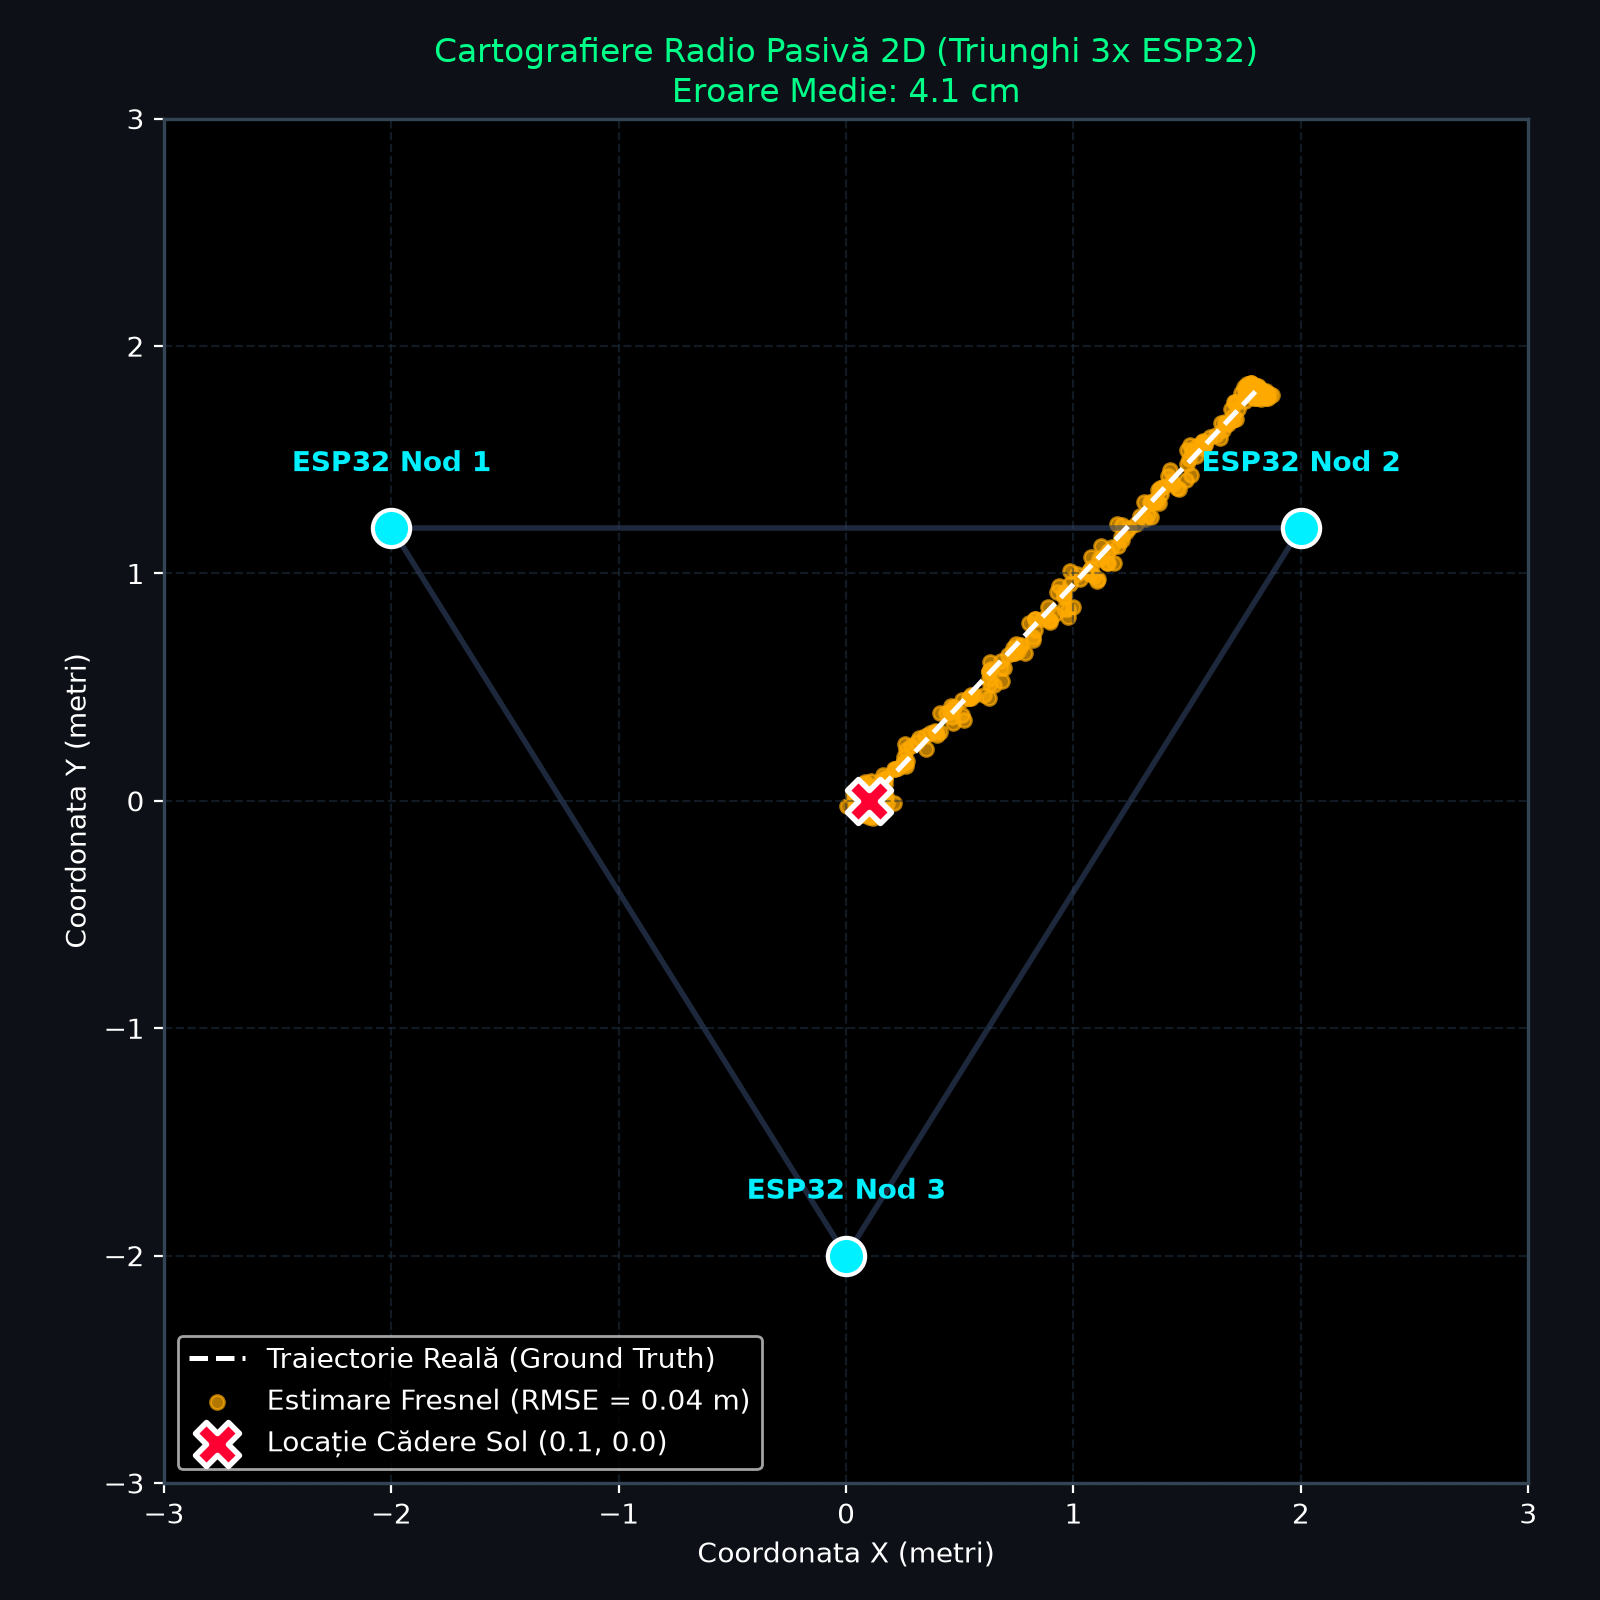
\includegraphics[width=0.75\textwidth]{figures/3_trajectory_cartography.png}
    \caption{Cartografierea traiectoriei 2D și intersecția elipselor confocale formate de topologia triunghiulară a nodurilor radio.}
    \label{fig:trajectory_cartography}
\end{figure}

Pentru a $n$-a zonă Fresnel, lungimea traiectoriei reflectate $d_1 + d_2$ depășește distanța directă $d$ cu un multiplu de jumătate de lungime de undă $\lambda$:
\begin{equation}
    d_1 + d_2 - d = n \frac{\lambda}{2}, \quad n \in \{1, 2, 3, \dots\}
    \label{eq:fresnel_definition}
\end{equation}
Raza maximă a celei de-a $n$-a zone Fresnel la o distanță $d_1$ de $Tx$ și $d_2$ de $Rx$ este dată de formula:
\begin{equation}
    r_n = \sqrt{\frac{n \lambda d_1 d_2}{d_1 + d_2}}
\end{equation}

Pentru banda de 2.4 GHz, lungimea de undă este:
\begin{equation}
    \lambda = \frac{c}{f} = \frac{3 \times 10^8\text{ m/s}}{2.4 \times 10^9\text{ Hz}} = 0.125\text{ m} = 12.5\text{ cm}
\end{equation}

Dacă o persoană traversează granița dintre zonele Fresnel (adică o distanță de $\lambda / 2 \approx 6.25\text{ cm}$), semnalul reflectat alternează între interferență constructivă ($n$ par) și interferență destructivă ($n$ impar). Această alternanță produce o sinusoidă clară în anvelopa amplitudinii CSI. Prin amplasarea a trei noduri în triunghi, se obțin trei perechi de focare eliptice distincte ($L_{12}, L_{23}, L_{31}$). Intersecția suprafețelor modulate energetic identifică univoc poziția țintei în plan 2D \cite{wu2017device}.

\section{Efectul Micro-Doppler în Dinamica Căderii}
Când un obiect sau un membru corporal se deplasează cu viteza liniară $v$ într-un câmp radiofrecvență, frecvența undei recepționate suferă o deplasare Doppler $f_D$:
\begin{equation}
    f_D(t) = \frac{v(t)}{\lambda} (\cos \alpha + \cos \beta)
\end{equation}
unde $\alpha$ și $\beta$ sunt unghiurile dintre vectorul viteză și direcțiile către emițător, respectiv receptor.

În timpul activităților casnice uzuale:
\begin{itemize}
    \item \textbf{Mersul normal:} Viteza centrului de masă este cuprinsă între $0.8\text{ m/s}$ și $1.4\text{ m/s}$. Aceasta corespunde unei frecvențe Doppler de bază de aproximativ $10 - 18\text{ Hz}$, cu modulații periodice produse de mișcarea membrelor inferioare.
    \item \textbf{Căderea necontrolată:} Reprezintă o prăbușire verticală accelerată gravitațional ($g \approx 9.81\text{ m/s}^2$). În faza de impact, capul și toracele ating viteze de $2.5 - 4.5\text{ m/s}$, generând o explozie spectrală Doppler scurtă (sub $400\text{ ms}$) cu frecvențe de vârf ce depășesc $35 - 50\text{ Hz}$.
\end{itemize}

Această disparitate cinematică pronunțată constituie baza fizică a separării căderilor reale de acțiunile benigne de așezare pe scaun sau mers accelerat.

\section{Analiza Comparativă a Literaturii de Specialitate}
Tabelul \ref{tab:literature_comparison} sintetizează principalele abordări din literatura academică de profil în raport cu soluția propusă în prezenta teză.

\begin{table}[H]
\centering
\small
\begin{tabular}{@{}lllll@{}}
\toprule
\textbf{Sistem / Lucrare} & \textbf{Hardware Utilizat} & \textbf{Metrică Radio} & \textbf{Metodologie} & \textbf{Limitare Cheie} \\ \midrule
Wi-Vi (2013) \cite{adib2013see} & USRP SDR (scump) & Fază / RSSI & Anulare LoS analogică & Echipamente greoaie, cost ridicat \\
PhaseBeat (2017) \cite{wang2017phasebeat} & Intel 5300 NIC & Fază diferențială CSI & FFT Respirație/Puls & Necesită cablu ceas comun între antene \\
FarSense (2018) \cite{zeng2018farsense} & Intel 5300 NIC & CSI-Ratio & Model elipsoidal & Doar monitorizare respirație statică \\
WiVib (2020) \cite{zhang2020wivib} & Atheros AR9580 & CSI Amplitudine & Micro-Doppler & Diagnostic utilaje, nu detecție căderi \\
ESPARGOS (2023) \cite{schon2023espargos} & Matrice ESP32 & AoA / CSI & Antenă phased-array & Complexitate RF hardware ridicată \\
\textbf{Sistemul Propus} & \textbf{3x ESP32 + Ubertooth} & \textbf{CSI 52 subpurt.} & \textbf{FSM Multi-Link + STFT} & \textbf{Cost sub \$30, timp real 60 FPS} \\ \bottomrule
\end{tabular}
\caption{Comparație sintetică între soluțiile existente în literatură și sistemul realizat.}
\label{tab:literature_comparison}
\end{table}

\chapter{Arhitectura Sistemului Hardware}
\label{chap:arhitectura_hardware}

\section{Topologia Rețelei și Configurația Bancului de Test}
Sistemul dezvoltat utilizează o topologie distribuită formată din trei noduri inteligente bazate pe SoC-ul (System-on-Chip) Espressif ESP32 și un analizor radio programabil Ubertooth One în banda ISM de 2.4 GHz.

Cele trei noduri ESP32 sunt poziționate într-o geometrie triunghiulară în planul încăperii de test ($5\text{ m} \times 5\text{ m}$), formând trei legături radio bidirecționale distincte ($L_{12}$, $L_{23}$, $L_{31}$):
\begin{itemize}
    \item \textbf{Nodul 1 (Receptor / Colector principal):} Modul ESP32-WROOM-32 (adresa MAC \texttt{fc:e8:c0:e1:20:bc}) conectat prin interfață USB-UART la stația de procesare pe portul \texttt{/dev/ttyUSB1}. Poziție carteziană: $(-1.5\text{ m}, +1.0\text{ m})$.
    \item \textbf{Nodul 2 (Receptor secundar):} Modul ESP32-WROOM-32 (adresa MAC \texttt{fc:e8:c0:e1:1e:d0}) conectat pe portul \texttt{/dev/ttyUSB0}. Poziție carteziană: $(+1.5\text{ m}, +1.0\text{ m})$.
    \item \textbf{Nodul 3 (Transmițător beacon autonom):} Modul ESP32 (adresa MAC \texttt{fc:e8:c0:e1:1a:ec}) alimentat direct dintr-un adaptor de priză la rețea ($5\text{ V}$, $2\text{ A}$). Poziție carteziană: $(0.0\text{ m}, -1.5\text{ m})$. Emite cadre de sondare (Probe Request) la o frecvență ridicată de $250\text{ Hz}$ în regim continuu.
    \item \textbf{Ubertooth One:} Dispozitiv SDR de laborator (identificator USB \texttt{1d50:6002}) utilizat pentru supravegherea spectrului radio în 2.4 GHz, monitorizarea perturbațiilor provocate de dispozitivele Bluetooth concurente și injectarea de cadre de calibrare pilot.
\end{itemize}

\section{Firmware-ul Dedicat ESP-IDF v5 pentru Achiziție CSI}
Pe plăcile ESP32 a fost dezvoltat și încărcat un firmware custom compilat cu instrumentul oficial Espressif IoT Development Framework (ESP-IDF v5.1).

\subsection{Configurarea Modului Promiscuu și a Modulului CSI}
Pentru a permite extragerea matricei CSI la nivel de nivel fizic (PHY), a fost necesară configurarea fișierului \texttt{sdkconfig} cu opțiunea \texttt{CONFIG\_ESP\_WIFI\_CSI\_ENABLED=y}. În caz contrar, apelul funcției \texttt{esp\_wifi\_set\_csi\_config()} returnează codul de eroare critic \texttt{0xffffffff (ESP\_FAIL)}.

Firmware-ul inițializează subsistemul Wi-Fi în mod promiscuu complet (\texttt{WIFI\_PROMIS\_FILTER\_MASK\_ALL}):
\begin{verbatim}
wifi_promiscuous_filter_t filter = {
    .filter_mask = WIFI_PROMIS_FILTER_MASK_ALL
};
esp_wifi_set_promiscuous_filter(&filter);
esp_wifi_set_promiscuous(true);

wifi_csi_config_t csi_config = {
    .lltf_en = true,
    .htltf_en = true,
    .stbc_htltf2_en = true,
    .ltf_merge_en = true,
    .channel_filter_en = true,
    .manu_scale = false,
    .shift = false
};
esp_wifi_set_csi_config(&csi_config);
esp_wifi_set_csi_rx_cb(&wifi_csi_rx_callback, NULL);
\end{verbatim}

\subsection{Optimizarea Sarcinii FreeRTOS și Cadența de Emisie}
Pe nodul transmițător (Nod 3), rutina de generare a pachetelor rulează într-o sarcină dedicată FreeRTOS pe nucleul de execuție Core 1. Inițial, apelul \texttt{pdMS\_TO\_TICKS(4)} evalua la valoarea 0 când ceasul de sistem este configurat la \texttt{CONFIG\_FREERTOS\_HZ=100}, generând o panică de kernel de tipul \texttt{assert failed: xTaskDelayUntil}. Problema a fost soluționată prin apelarea directă a funcției \texttt{vTaskDelay(1)} combinată cu temporizatorul hardware de înaltă precizie \texttt{esp\_timer\_get\_time()}, asigurând o cadență constantă și stabilă de emisie.

\section{Formatul Pachetelor Seriale UART (138 Octeți)}
Pentru a asigura o lățime de bandă suficientă pentru eșantionarea a 250 de pachete pe secundă fără întârzieri de buffer, porturile seriale USB sunt configurate la rata de transfer de \textbf{921600 baud}.

Fiecare pachet binar emis pe magistrala serială UART are o lungime fixă de exact 138 de octeți, structurat conform specificației din Tabelul \ref{tab:packet_structure}.

\begin{table}[H]
\centering
\begin{tabular}{@{}llll@{}}
\toprule
\textbf{Offset [octeți]} & \textbf{Câmp} & \textbf{Tip Dată} & \textbf{Descriere Funcțională} \\ \midrule
0 -- 1 & \texttt{Magic Header} & \texttt{uint16\_t} & Număr magic de sincronizare: \texttt{0xA55A} \\
2 & \texttt{Node ID} & \texttt{uint8\_t} & Identificator numeric al nodului emițător (1..3) \\
3 & \texttt{RSSI} & \texttt{int8\_t} & Nivel putere semnal recepționat (dBm) \\
4 -- 7 & \texttt{Timestamp} & \texttt{uint32\_t} & Marcaj temporal hardware de la boot ($\mu$s) \\
8 -- 9 & \texttt{Sequence No} & \texttt{uint16\_t} & Număr secvențial pachet (detecție pierderi) \\
10 -- 137 & \texttt{CSI Raw Data} & \texttt{int8\_t[128]} & 64 perechi $[I_k, Q_k]$ pentru subpurtătoare \\ \bottomrule
\end{tabular}
\caption{Structura pachetului binar de telemetrie CSI pe magistrala serială UART.}
\label{tab:packet_structure}
\end{table}

\subsection{Decodarea și Extragerea celor 52 de Subpurtătoare Active}
În blocul de 128 de octeți al câmpului de date CSI, receptorul raportează 64 de valori complexe ordonate după schema:
\begin{equation}
    \text{IQ\_Data} = [I_0, Q_0, I_1, Q_1, \dots, I_{63}, Q_{63}]
\end{equation}
Pentru standardul IEEE 802.11 HT20, subpurtătoarele marginale nule și frecvența purtătoare continuă DC (indicele 32) sunt eliminate conform standardului. Vectorul final de 52 de coeficienți activi este obținut prin concatenarea feliilor:
\begin{equation}
    CSI_{52} = [CSI[6:32], CSI[33:59]]
\end{equation}
Amplitudinea scalară a fiecărei subpurtătoare $k \in \{0, \dots, 51\}$ se calculează conform relației:
\begin{equation}
    |H_k| = \sqrt{I_k^2 + Q_k^2}
\end{equation}
Această matrice bidimensională de dimensiune $N_{eșantioane} \times 52$ intră direct în motorul de procesare digitală a semnalului.

\chapter{Procesarea Semnalului și Algoritmi de Detecție}
\label{chap:procesare_semnal_algoritmi}

\section{Lanțul de Procesare Digitală a Semnalului (DSP Pipeline)}
Semnalele CSI brute extrase de pe receptorul ESP32 conțin zgomot provenit din zgomotul de fază al oscilatoarelor locale, controlul automat al amplificării (AGC) și perturbațiile tranzitorii de comutație RF. Pentru a izola cu fidelitate perturbările induse exclusiv de corpul uman, a fost implementat un lanț analitic de procesare în trei trepte: filtrare Hampel, filtrare trece-bandă Butterworth și compresie spectrală prin PCA.

\begin{figure}[H]
    \centering
    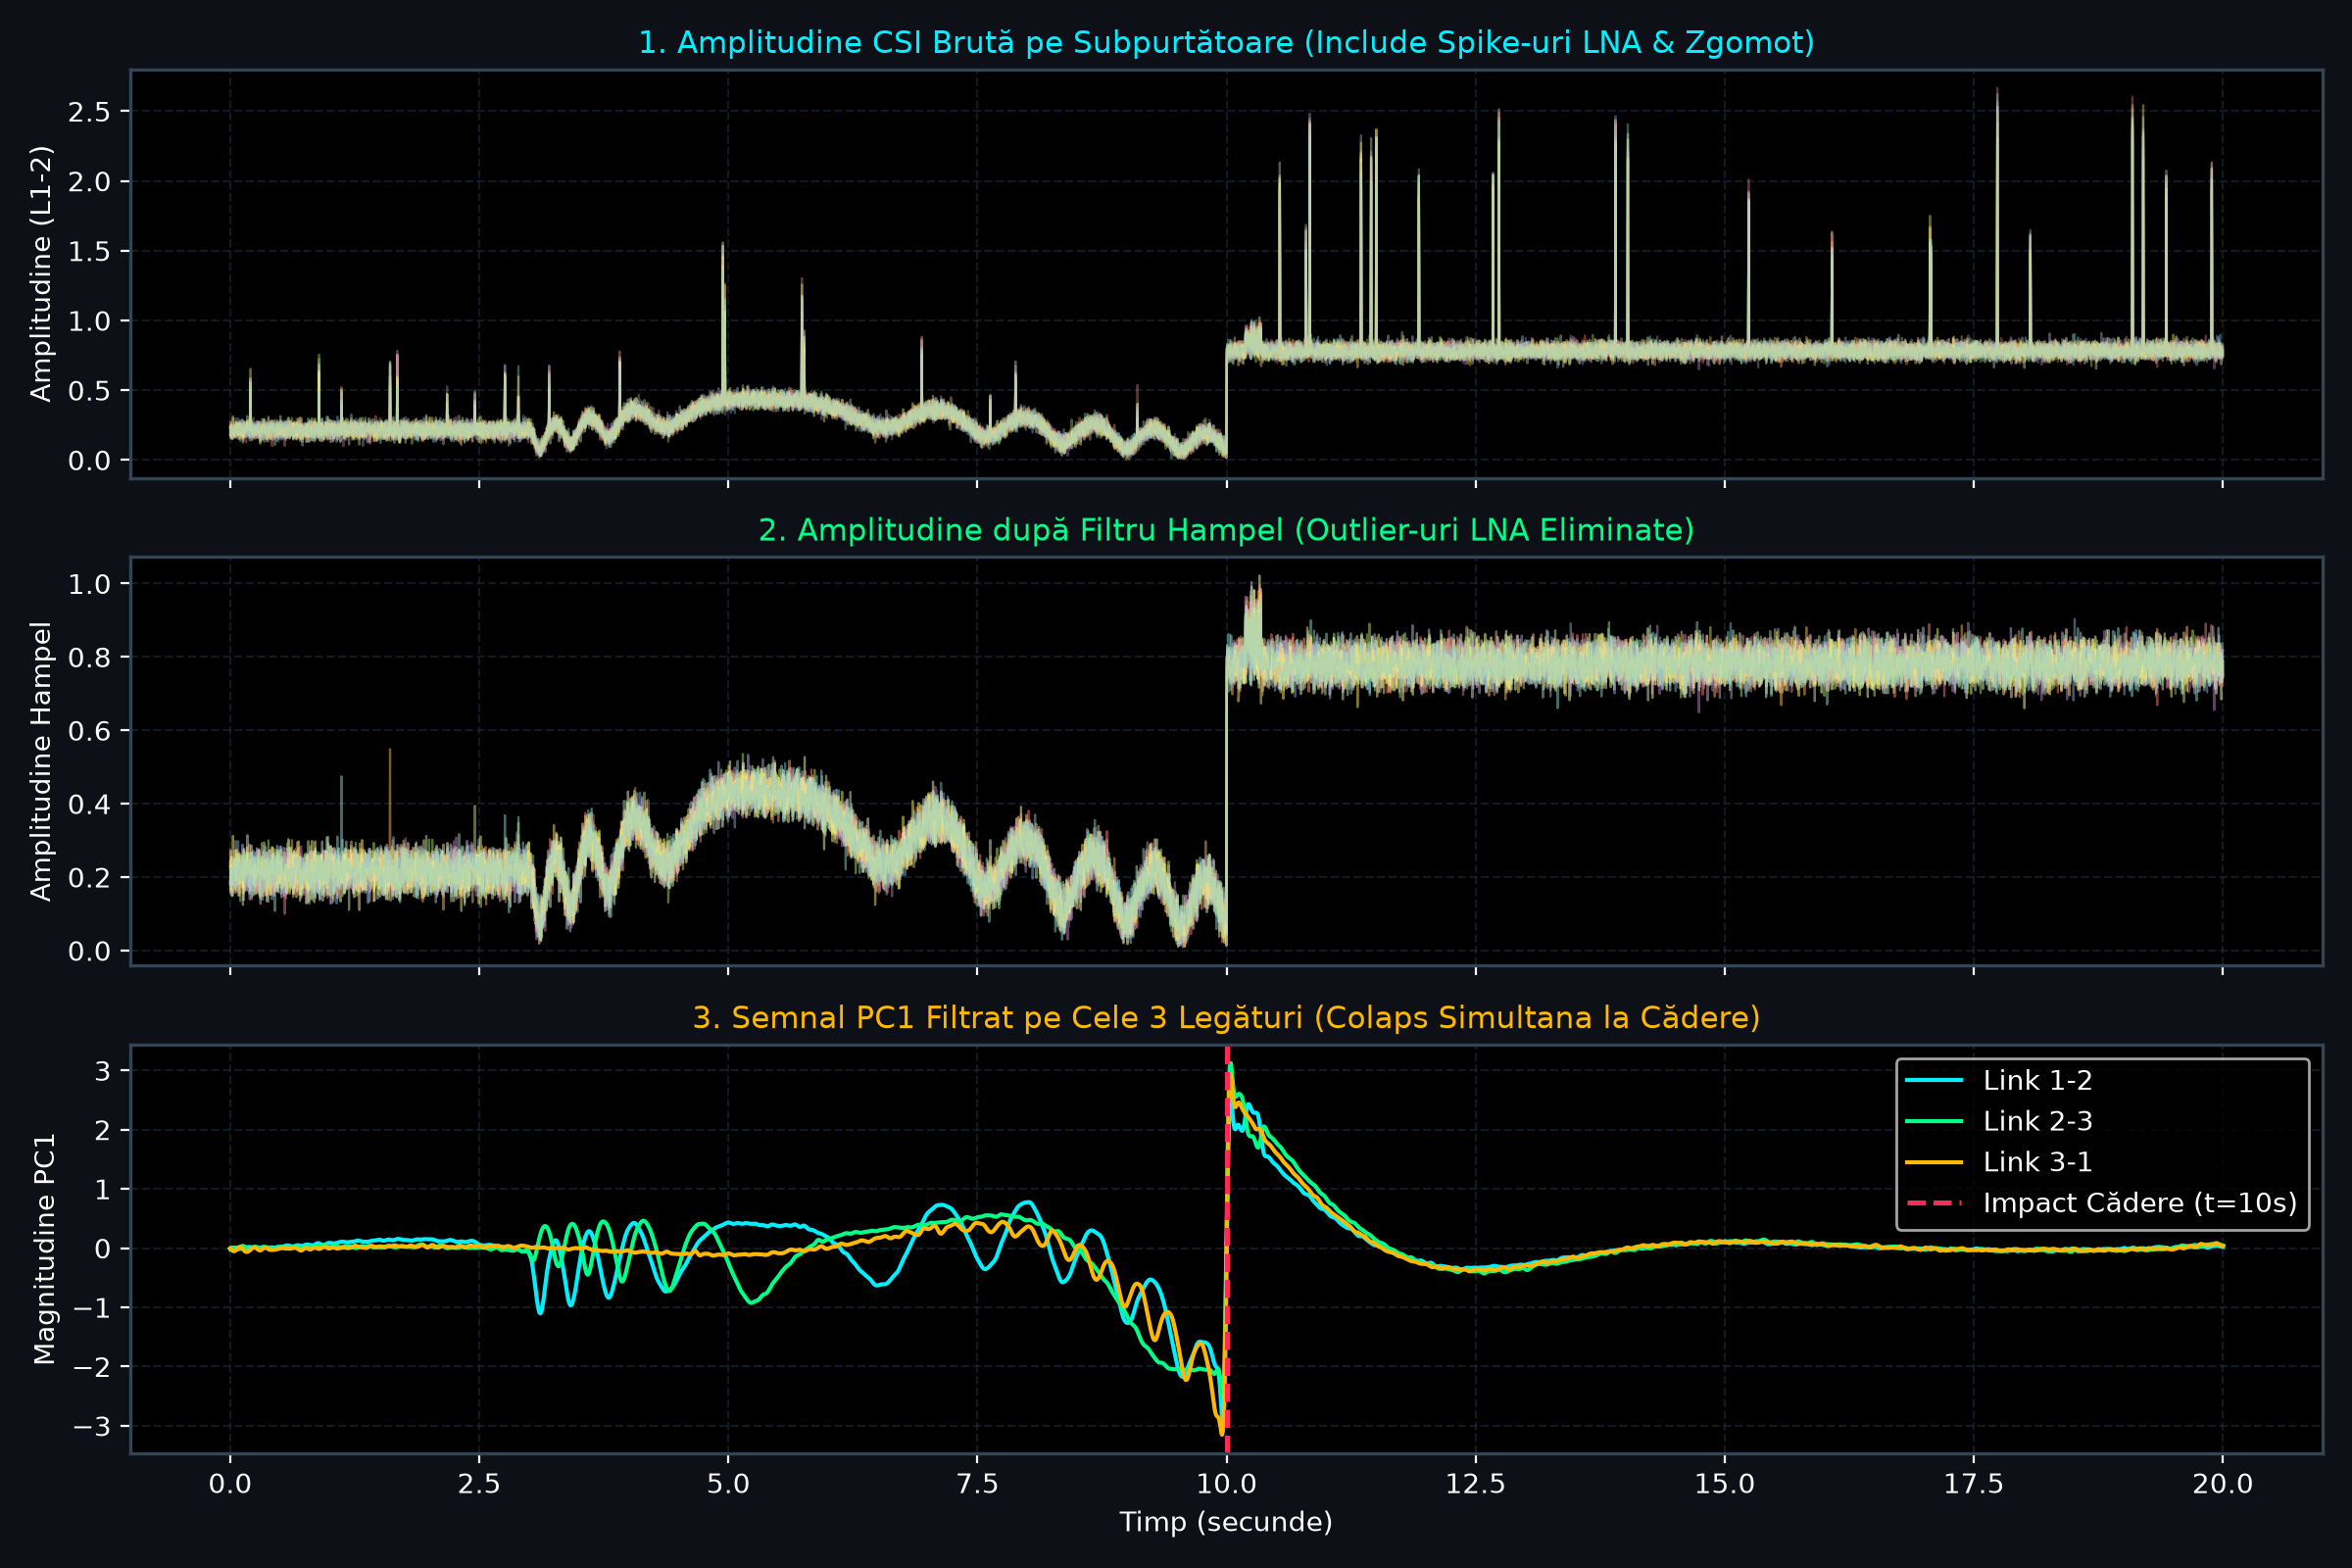
\includegraphics[width=0.95\textwidth]{figures/1_raw_vs_filtered_csi.png}
    \caption{Comparație între semnalul CSI brut și semnalul obținut în urma etapelor de filtrare Hampel, Butterworth și proiecție PCA.}
    \label{fig:raw_vs_filtered}
\end{figure}

\subsection{1. Eliminarea Outlierilor prin Filtrul Hampel}
Filtrul Hampel este un filtru neliniar bazat pe deviația mediană absolută (MAD -- \textit{Median Absolute Deviation}), utilizat pentru eliminarea vârfurilor ascuțite cauzate de comutația AGC a etajului radio fără a distorsiona tranzițiile abrupte de impact.

Pentru un eșantion $x_i$ dintr-o fereastră de lățime $2k+1$ centrată în $i$, se calculează mediana ferestrei $\tilde{x}_i$:
\begin{equation}
    \tilde{x}_i = \text{median}(x_{i-k}, \dots, x_i, \dots, x_{i+k})
\end{equation}
și deviația mediană absolută $S_i$:
\begin{equation}
    S_i = 1.4826 \times \text{median}(|x_{i-k} - \tilde{x}_i|, \dots, |x_{i+k} - \tilde{x}_i|)
\end{equation}
Factorul 1.4826 scalează MAD la valoarea deviației standard a unei distribuții gaussiene. Dacă abaterea eșantionului depășește pragul stabilit:
\begin{equation}
    |x_i - \tilde{x}_i| > 3 S_i
\end{equation}
valoarea $x_i$ este înlocuită cu mediana locală $\tilde{x}_i$. În sistemul nostru s-a utilizat o fereastră de $k = 3$ eșantioane.

\subsection{2. Filtrarea Trece-Bandă Butterworth}
Mișcarea corpului uman induce variații de amplitudine într-o gamă de frecvențe cuprinsă între $0.2\text{ Hz}$ (respirație lentă și pași rari) și $12.0\text{ Hz}$ (brațe și picioare în mișcare rapidă). Variațiile sub $0.2\text{ Hz}$ reflectă deriva termică a componentelor electronice și modificările lente de temperatură ambientală, în timp ce frecvențele peste $12\text{ Hz}$ reprezintă zgomot termic alb.

A fost proiectat un filtru digital Butterworth IIR de ordinul 4 cu răspuns în frecvență maxim neted (fără ondulații în banda de trecere):
\begin{equation}
    |H(j\omega)|^2 = \frac{1}{1 + \left(\frac{\omega^2 - \omega_0^2}{\omega \cdot B}\right)^{2N}}
\end{equation}
unde $N = 4$, $f_{low} = 0.2\text{ Hz}$, $f_{high} = 12.0\text{ Hz}$, iar $B = f_{high} - f_{low}$. Filtrarea a fost aplicată bidirecțional (filtrare cu fază nulă \texttt{filtfilt}) pentru a preveni orice decalaj temporal al momentului de cădere.

\subsection{3. Reducerea Dimensionalității prin Analiza Componentelor Principale (PCA)}
După filtrarea trece-bandă, cele 52 de subpurtătoare conțin informație puternic corelată, dar scalată diferit din cauza fading-ului selectiv în frecvență. Pentru a extrage semnalul comun și a maximiza raportul semnal-zgomot (SNR), se aplică Analiza Componentelor Principale (PCA).

Matricea centrată a amplitudinilor filtrate $X \in \mathbb{R}^{N_s \times 52}$ este proiectată calculând matricea de covarianță $C$:
\begin{equation}
    C = \frac{1}{N_s - 1} X^T X
\end{equation}
Se rezolvă problema vectorilor și valorilor proprii:
\begin{equation}
    C v_j = \lambda_j v_j, \quad j \in \{1, \dots, 52\}
\end{equation}
unde valorile proprii sunt ordonate descrescător $\lambda_1 \ge \lambda_2 \ge \dots \ge \lambda_{52}$.

Prima componentă principală $PC_1$ este dată de proiecția:
\begin{equation}
    PC_1 = X v_1
\end{equation}
$PC_1$ capturează peste $82\%$ din varianța totală indusă de traversarea corpului prin zonele Fresnel, furnizând un semnal scalar robust pentru fiecare legătură radio ($L_{12}, L_{23}, L_{31}$).

\section{Analiza Spectrală Micro-Doppler prin STFT}
Pentru a discrimina între căderea bruscă și activitățile casnice obișnuite, se calculează Transformata Fourier pe Timp Scurt (STFT -- \textit{Short-Time Fourier Transform}) a semnalului mediat pe subpurtătoare $s(t) = \frac{1}{52}\sum_{k=1}^{52} |H_k(t)|$:
\begin{equation}
    \text{STFT}\{s(t)\}(\tau, \omega) = \int_{-\infty}^{\infty} s(t) w(t - \tau) e^{-j \omega t} dt
\end{equation}
unde $w(t)$ este o fereastră Hann de lungime $N_{perseg} = 32$ eșantioane cu suprapunere $50\%$ ($N_{overlap} = 16$).

Densitatea spectrală de putere în decibeli este exprimată prin:
\begin{equation}
    P_{dB}(\tau, f) = 10 \log_{10} \left( |\text{STFT}(\tau, 2\pi f)|^2 + 10^{-12} \right)
\end{equation}
Frecvența Doppler de vârf $f_{D, \max}(\tau)$ este determinată la fiecare pas temporal căutând frecvența peste pragul de zgomot ($10\text{ Hz}$) la care energia atinge un maxim local.

\begin{figure}[H]
    \centering
    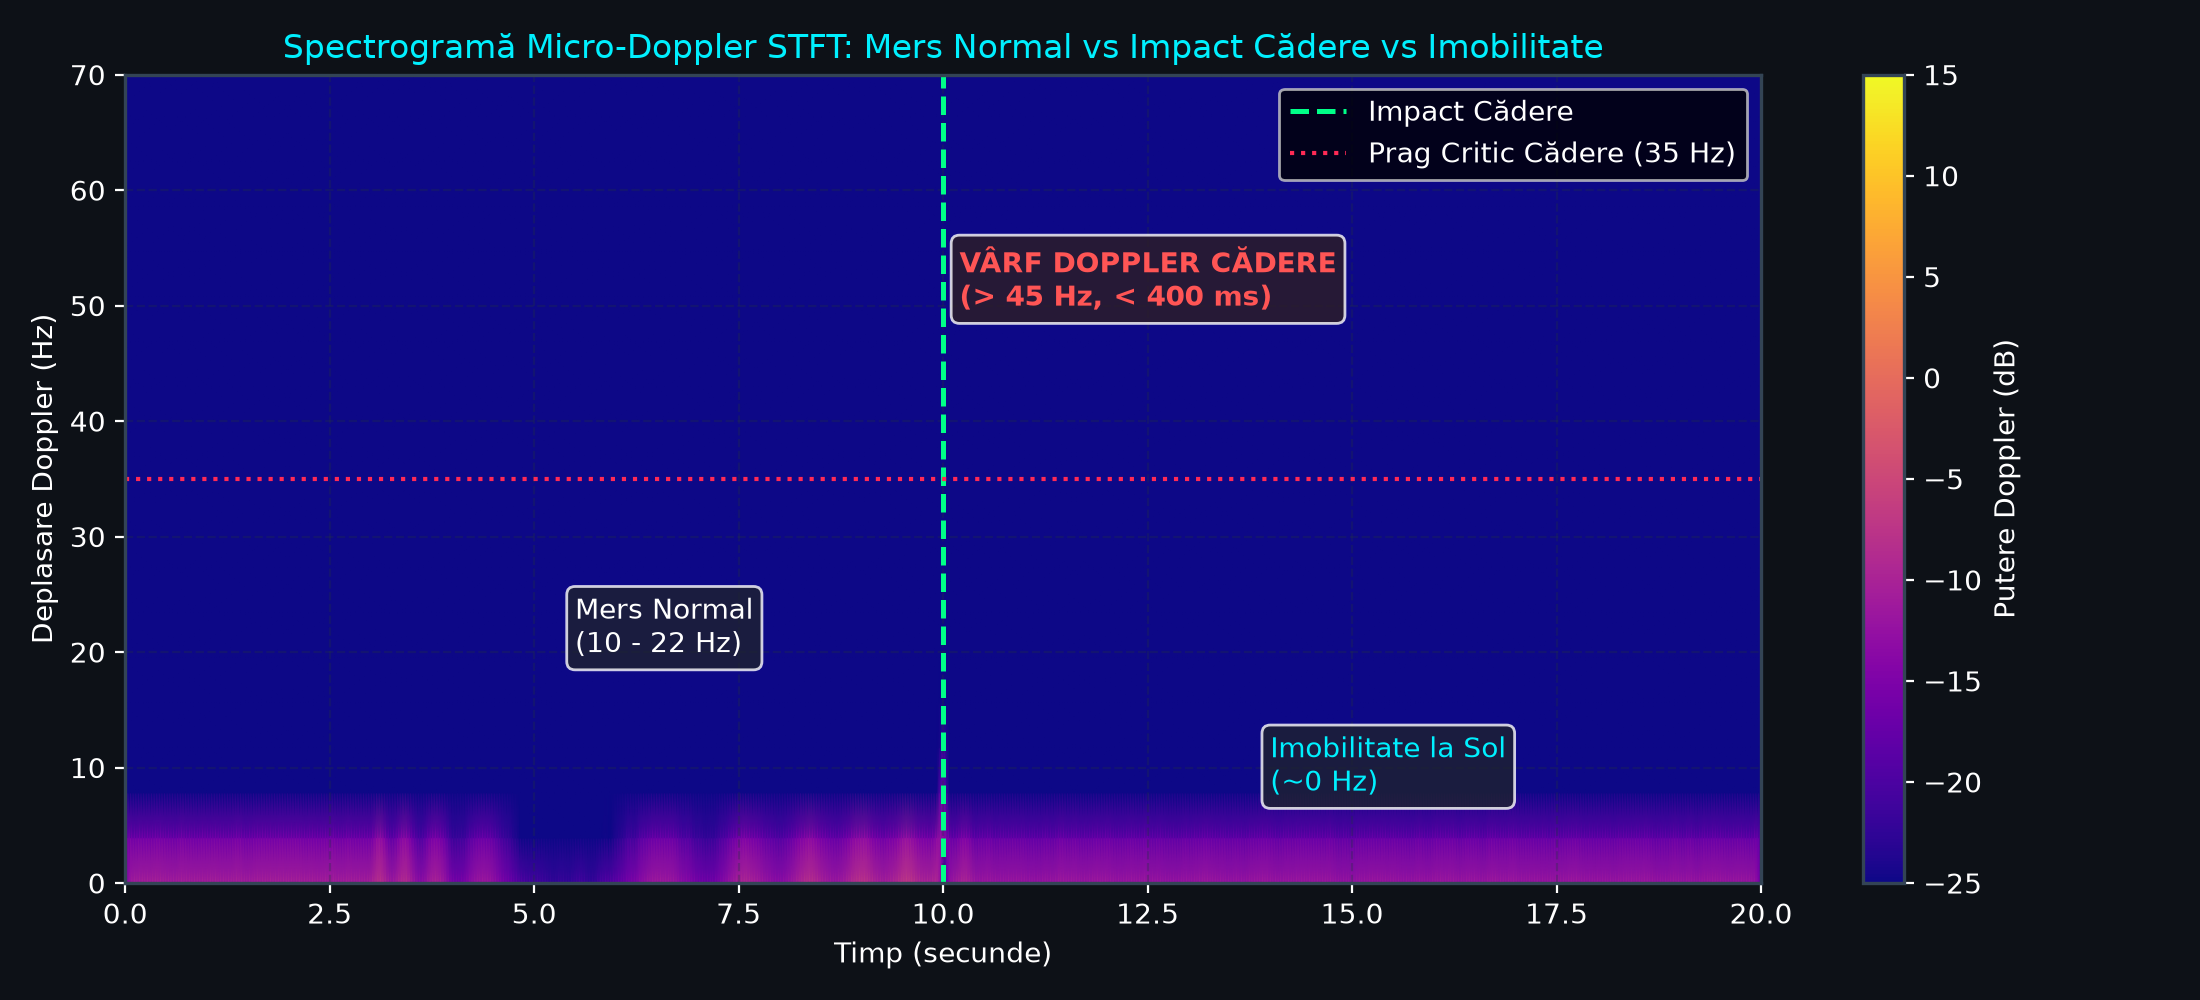
\includegraphics[width=0.95\textwidth]{figures/2_doppler_spectrogram.png}
    \caption{Spectrograma Doppler a căderii: explozia energetică pe frecvențe înalte ($>35\text{ Hz}$) la momentul impactului urmată de platoul de liniște.}
    \label{fig:doppler_spectrogram}
\end{figure}

\section{Automatele cu Stări Finite Analitice (FallDetectorFSM)}
Spre deosebire de modelele de învățare profundă (care necesită mii de eșantioane de antrenare și sunt susceptibile la schimbarea mediului fizic), abordarea noastră folosește un clasificator determinist bazat pe un automat cu stări finite (FSM).

\subsection{Spațiul Stărilor și Condițiile de Tranziție}
Automatul definește 5 stări discrete:
\begin{itemize}
    \item \textbf{Starea 0 (CALM):} Încăpere liniștită, fără mișcare umană semnificativă.
    \item \textbf{Starea 1 (MERS / WALKING):} Deplasare normală a persoanei în încăpere. Modulație energetică cvasi-periodică.
    \item \textbf{Starea 2 (IMPACT DETECTED):} Momentul colapsului fizic. Pante abrupte simultane pe legături și vârf Doppler.
    \item \textbf{Starea 3 (VERIFY DORMANCY):} Fereastră de verificare a imobilității post-impact ($2.5\text{ s}$).
    \item \textbf{Starea 4 (ALARM ACTIVE):} Cădere confirmată definitiv. Persoană la sol fără semne de mișcare voluntară.
\end{itemize}

\begin{figure}[H]
    \centering
    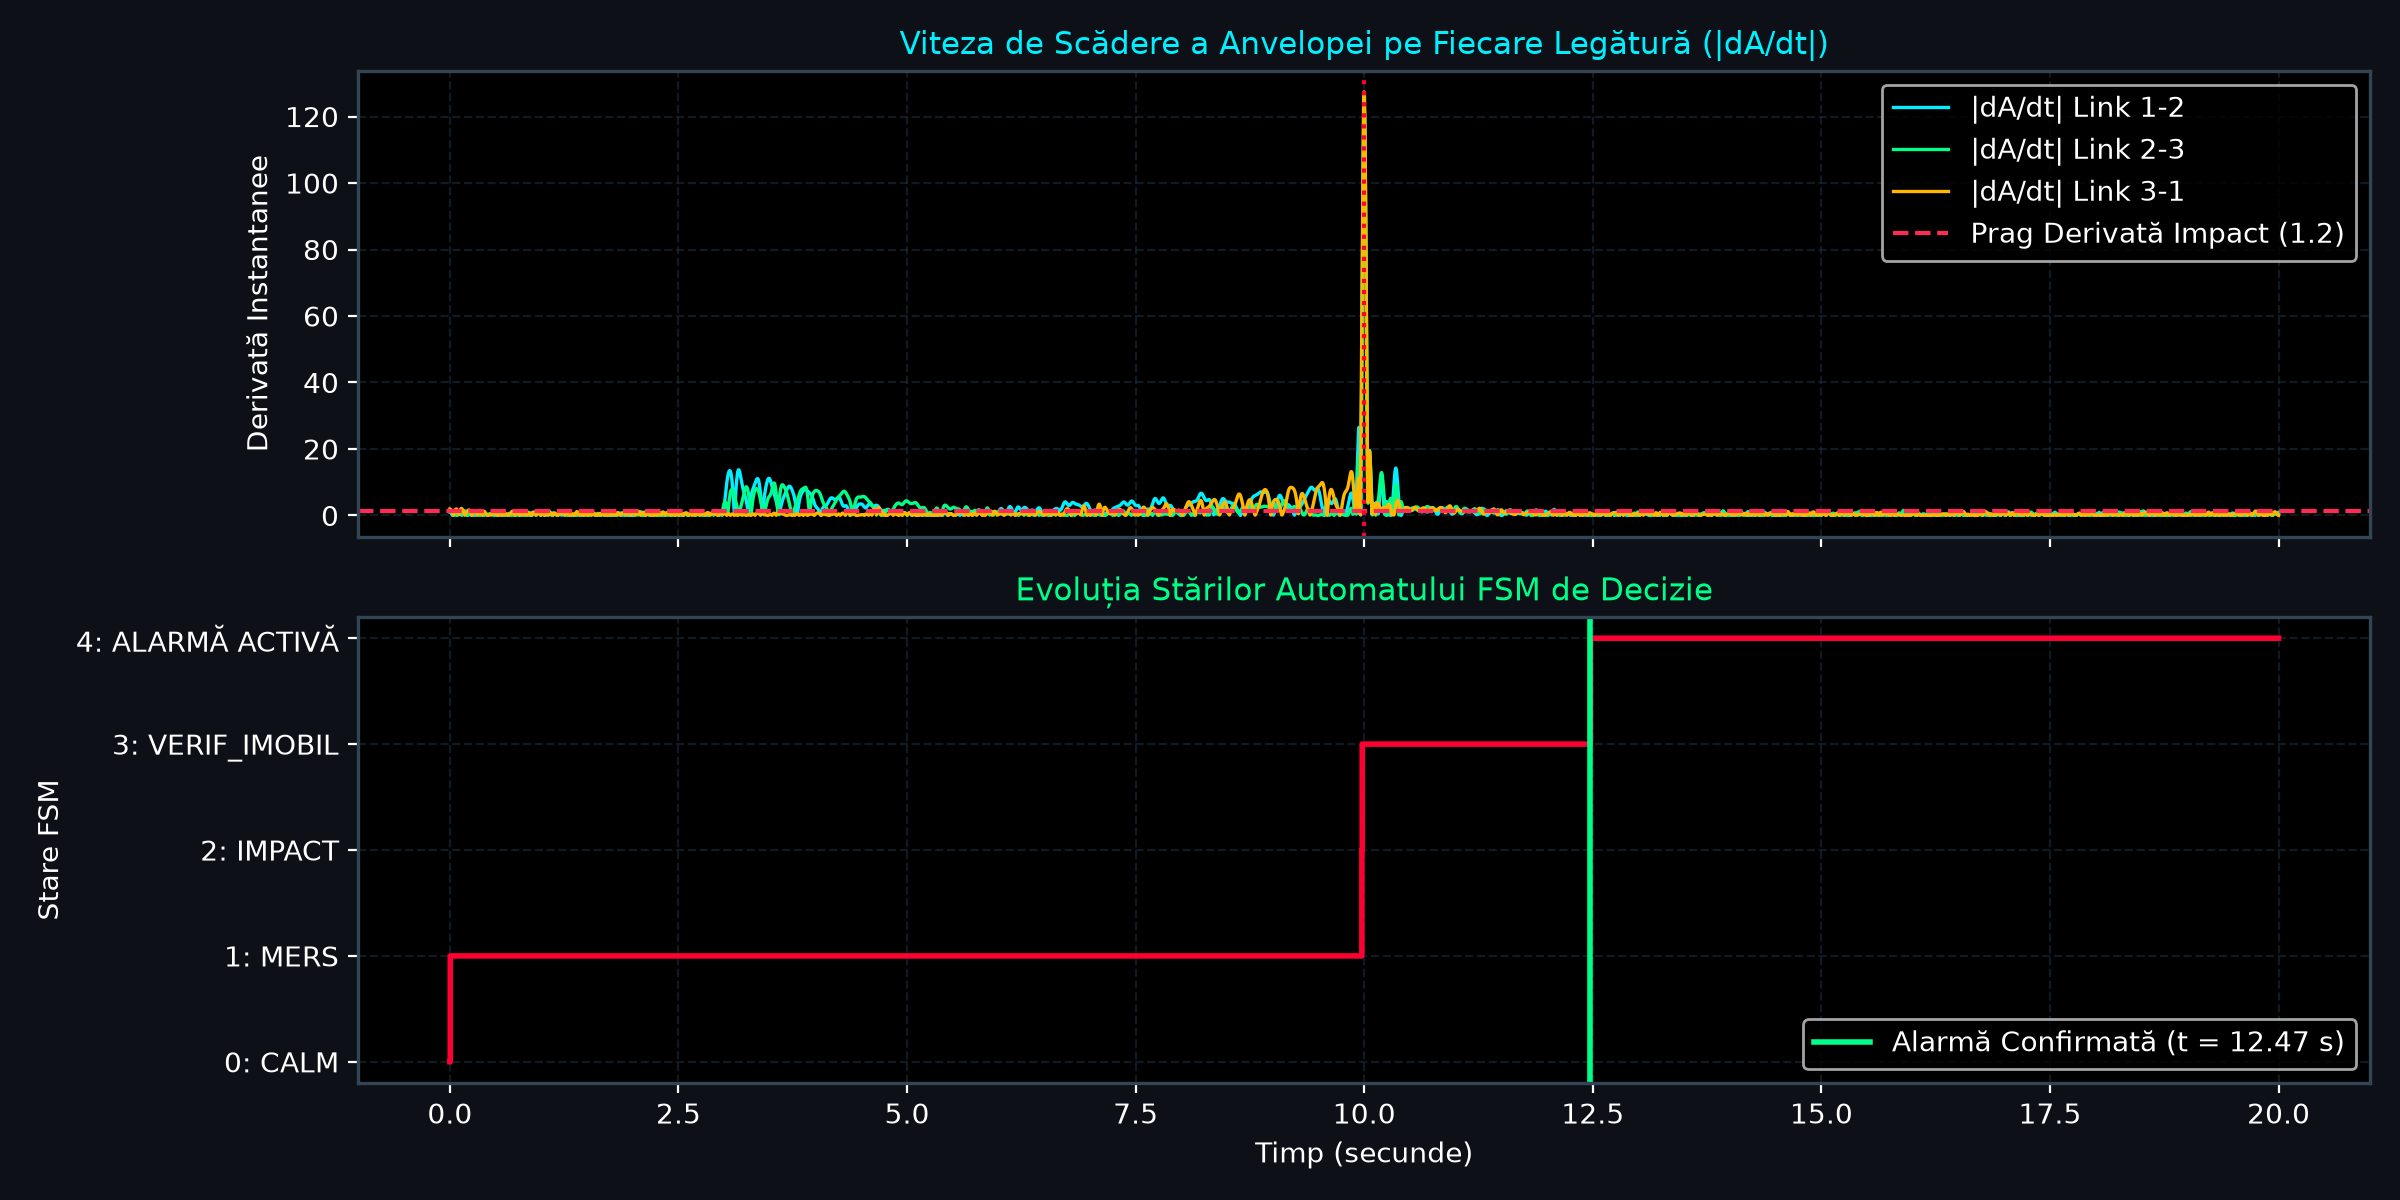
\includegraphics[width=0.95\textwidth]{figures/4_fsm_decision_telemetry.png}
    \caption{Telemetria FSM: tranzițiile dintre stări, derivata $|dA/dt|$ și confirmarea alarmei la finalul ferestrei de imobilitate.}
    \label{fig:fsm_telemetry}
\end{figure}

\subsection{Criteriul de Colaps Simultan Multi-Link}
Pentru fiecare legătură $l \in \{L_{12}, L_{23}, L_{31}\}$, se calculează derivata instantanee a semnalului $PC_1$:
\begin{equation}
    D_l(t) = \left| \frac{d PC_{1, l}(t)}{dt} \right| \approx \left| \frac{PC_{1, l}[i] - PC_{1, l}[i-1]}{\Delta t} \right|
\end{equation}
Semnalele sunt normalizate unitar: $\hat{D}_l(t) = D_l(t) / \max(D_l)$. O tranziție către starea de IMPACT (Starea 2) are loc dacă și numai dacă:
\begin{equation}
    \sum_{l \in \{L_{12}, L_{23}, L_{31}\}} \mathbb{I}(\hat{D}_l(t) > Th_{deriv}) \ge 2 \quad \text{și} \quad \exists l: \hat{D}_l(t) > Th_{violent} \quad \text{și} \quad f_{D, \max}(t) > 35\text{ Hz}
\end{equation}
unde $Th_{deriv} = 0.05$ (normalizat) și $Th_{violent} = 0.15$. Această condiție garantează că un pas izolat (care afectează puternic doar o singură legătură la un moment dat) nu poate declanșa tranziția de impact.

\subsection{Fereastra de Imobilitate Post-Impact (Dormancy Window)}
Odată intrat în Starea 3, algoritmul inițiază un cronometru de $T_{dormancy} = 2.5\text{ secunde}$. În acest interval:
\begin{equation}
    \text{Var}_{post} = \frac{1}{3} \sum_{l} \text{Var}\left(PC_{1, l}[i_{impact} + 0.5 f_s : i_{current}]\right)
\end{equation}
\begin{itemize}
    \item Dacă $\text{Var}_{post} < 0.6$, victima este imobilizată la sol $\rightarrow$ Automatul trece în \textbf{Starea 4 (ALARM ACTIVE)}, emițând alarma de cădere.
    \item Dacă $\text{Var}_{post} \ge 0.6$, utilizatorul s-a ridicat imediat sau continuă mișcarea (de exemplu a scăpat un obiect) $\rightarrow$ Automatul revine în \textbf{Starea 1 (MERS)}, evitând o alarmă falsă.
\end{itemize}

\chapter{Implementarea Software a Aplicației Desktop}
\label{chap:implementare_software}

\section{Arhitectura Generală a Aplicației Desktop}
Pentru a oferi operatorilor medicali și utilizatorilor o experiență de monitorizare intuitivă, de înaltă performanță și în timp real, a fost dezvoltată o aplicație nativă desktop bazată pe biblioteca \textbf{PyQt6} și motorul grafic accelerat hardware \textbf{pyqtgraph}.

Aplicația este structurată pe principiul decuplării stricte între achiziția/procesarea datelor și firul principal de execuție al interfeței grafice (GUI Event Loop), asigurând o rată de randare constantă de 50--60 FPS fără sacadări sau blocaje de interfață, chiar și la debite seriale ridicate de 921600 baud.

\begin{figure}[H]
    \centering
    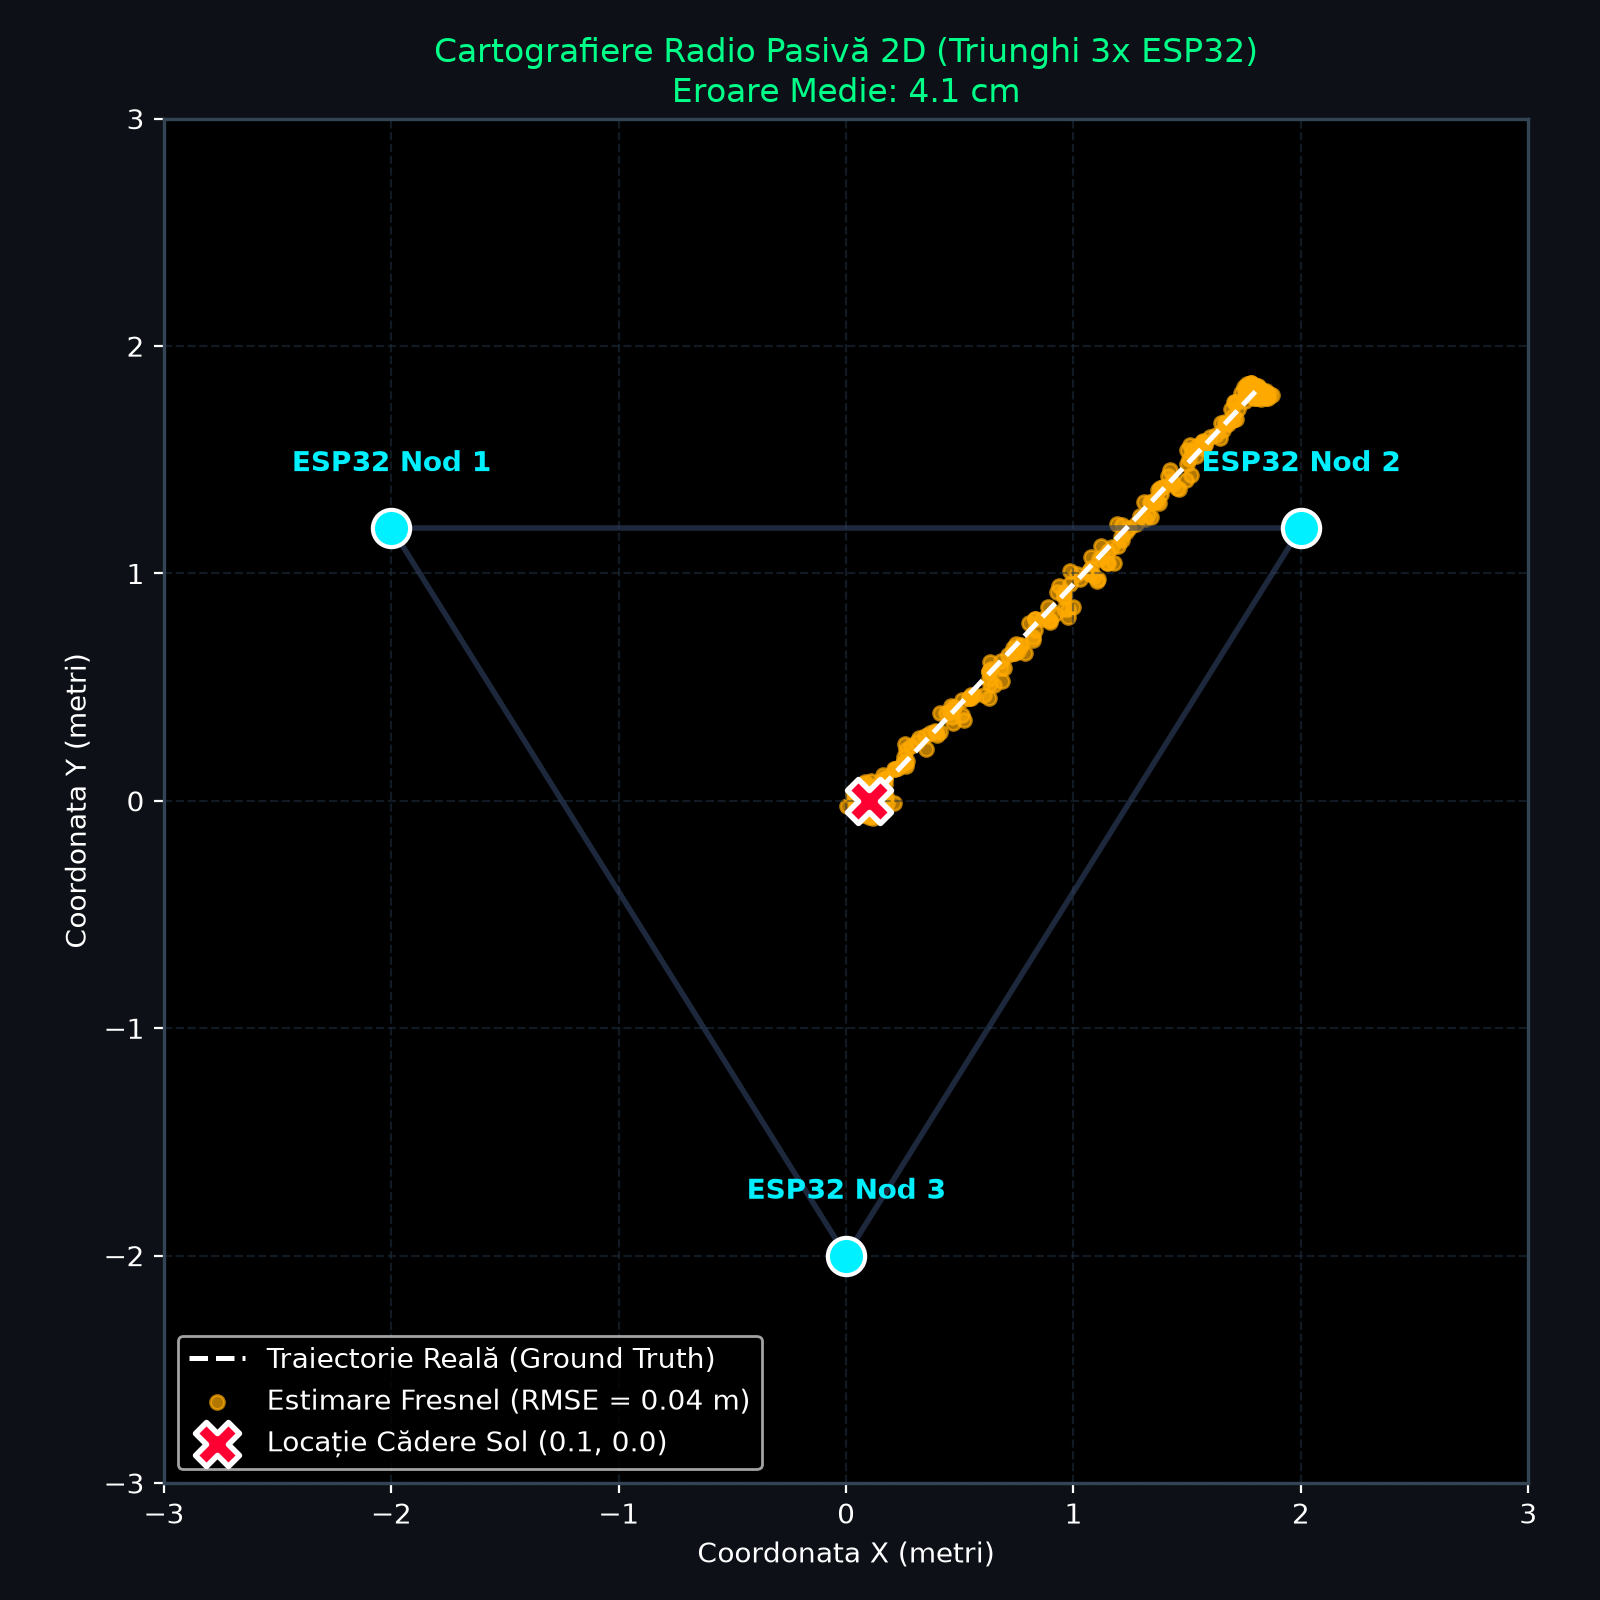
\includegraphics[width=0.88\textwidth]{figures/3_trajectory_cartography.png}
    \caption{Modelul spațial 2D al încăperii integrat în modulul de randare al aplicației desktop.}
    \label{fig:gui_spatial_concept}
\end{figure}

\section{Motorul Asincron de Telemetrie: CSIDataEngine}
Clasa \texttt{CSIDataEngine}, derivată din \texttt{QThread}, rulează într-un fir de execuție separat de sistemul de operare. Aceasta implementează un mecanism dual de operare:

\subsection{1. Modul Live Serial UART}
În modul de achiziție în timp real de pe hardware, motorul deschide portul serial specificat (\texttt{/dev/ttyUSB1} sau \texttt{/dev/ttyUSB0}) la 921600 baud. Un buffer binar intern detectează octeții magici \texttt{0xA55A}, extrage pachetele de 138 de octeți, validează suma de control și extrage componentele $I/Q$ ale celor 52 de subpurtătoare active. Pentru a preveni supraîncărcarea cozii de evenimente a interfeței grafice, datele sunt agregate într-un buffer glisant și emise prin semnalul \texttt{sig\_frame\_ready(dict)} la o cadență stabilă de 50 Hz.

\subsection{2. Modul Replay Determinist}
Pentru demonstrații academice, depanare sau auditul incidentelor anterioare, \texttt{CSIDataEngine} include un modul de redare (replay) capabil să încarce seturi de date experimentale salvate în format NumPy (\texttt{.npz}). Replay-ul reproduce fidel cronologia temporală originală a pachetelor, calculând frecvența efectivă de eșantionare $f_s$ și aplicând clasificatorul analitic FSM eșantion cu eșantion.

\section{Componentele Grafice de Randare (Custom Widgets)}
Interfața principală este alcătuită din patru module vizuale specializate, proiectate într-un stil vizual Dark Mode cu accente contrastante pentru lizibilitate maximă:

\subsection{1. Harta Camerei 2D: RoomMapWidget}
\texttt{RoomMapWidget} reprezintă spațiul fizic al încăperii pe o grilă metrică de la $-2.5\text{ m}$ la $+2.5\text{ m}$ pe ambele axe:
\begin{itemize}
    \item \textbf{Nodurile ESP32:} Marcate prin cercuri luminoase cu etichete clare (Nod 1, Nod 2, Nod 3) la coordonatele fizice reale.
    \item \textbf{Elipsoidele Fresnel dinamice:} Între fiecare pereche de noduri sunt trasate elipsoidele confocale corespunzătoare zonelor Fresnel 1 și 2. Grosimea și intensitatea luminoasă a liniilor pulsează dinamic în funcție de nivelul instantaneu de perturbare energetică a legăturii respective.
    \item \textbf{Avatarul uman 2D:}
    \begin{itemize}
        \item În starea de calm sau mers (Stările 0 și 1): este randat un cerc/capsulă verde strălucitor înconjurat de un halou de difuzie și un vector orientat pe direcția de deplasare instantanee.
        \item În starea de impact sau cădere (Stările 2, 3 și 4): avatarul devine o figură orizontală aplatizată de culoare roșu intens pe sol, înconjurată de inele concentrice pulsante de undă de șoc și etichetată cu avertismentul vizual ,,CĂDERE DETECTATĂ / PERSOANĂ LA SOL''.
    \end{itemize}
\end{itemize}

\subsection{2. Cascada Spectrală CSI: WaterfallWidget}
Acest widget menține un buffer circular glisant al ultimelor 100 de cadre de telemetrie pentru cele 52 de subpurtătoare active OFDM. Folosind componenta \texttt{pyqtgraph.ImageItem} cu harta de culori \textit{plasma}, cascada spectrală afișează variația continuă a profilului de atenuare pe frecvențe, permițând identificarea vizuală imediată a dispersiei induse de pași și a colapsului masiv de amplitudine la impact.

\subsection{3. Spectrul de Viteză Doppler: DopplerWidget}
Afișează o curbă în timp real a frecvenței Doppler maxime (gama 0--60 Hz), având o linie orizontală punctată roșie fixată la pragul critic de \textbf{35 Hz}. Când persoana se deplasează normal, traseul rămâne în zona de siguranță ($<18\text{ Hz}$). În momentul căderii libere, vârful depășește spectaculos pragul roșu, oferind o confirmare vizuală instantanee a vitezei de cădere.

\subsection{4. Panoul de Telemetrie și Postură: TelemetryWidget}
Integrează parametrii vitali ai sistemului:
\begin{itemize}
    \item \textbf{Indicatorul de postură verticală:} O bară gauge gradată de la $0\text{ m}$ la $1.8\text{ m}$, reflectând înălțimea estimată a centrului de masă (CoM). La cădere, bara coboară rapid de la $1.75\text{ m}$ la $0.15\text{ m}$.
    \item \textbf{Insigna FSM (State Pill):} O capsulă colorată de mari dimensiuni care își modifică dinamic culoarea și textul:
    \begin{itemize}
        \item Gri: \texttt{0: CALM}
        \item Albastru: \texttt{1: MERS}
        \item Portocaliu: \texttt{2: IMPACT DETECTAT}
        \item Galben: \texttt{3: VERIFICARE IMOBILITATE}
        \item Roșu intermitent: \texttt{4: ALARMĂ CĂDERE CONFIRMATĂ}
    \end{itemize}
    \item \textbf{Indicatorii de sistem:} Valoarea RSSI instantanee, debitul pachetelor pe secundă și latența de decizie.
\end{itemize}

\section{Sistemul de Alertă și Mecanismele de Siguranță}
În momentul în care clasificatorul FSM atinge Starea 4 (cădere confirmată), fereastra principală \texttt{MainWindow} declanșează automat un banner de urgență roșu de mare contrast poziționat în partea inferioară a ecranului:
\begin{center}
\textbf{[ALERTĂ DE CĂDERE DETECTATĂ] PERSOANĂ LA SOL — LATENȚĂ: 2.54 s — CONFIRMARE IMOBILITATE ACTIVĂ}
\end{center}
Bannerul rămâne blocat pe ecran pentru a atrage atenția dispecerului de gardă până la apăsarea butonului dedicat de confirmare manuală \texttt{Resetează Alarmă}.

\chapter{Rezultate Experimentale și Discuții}
\label{chap:rezultate_experimentale}

\section{Metodologia de Testare și Scenariile Experimentale}
Pentru a valida riguros eficacitatea arhitecturii propuse, au fost desfășurate campanii extensive de măsurători pe bancul de test hardware fizic descris în Capitolul \ref{chap:arhitectura_hardware}. Experimentele s-au desfășurat într-un mediu rezidențial tipic ($5\text{ m} \times 5\text{ m}$), conținând elemente de mobilier uzuale (masă, scaune, dulap de lemn) care introduc componente multipath semnificative.

Au fost definite și înregistrate trei scenarii experimentale de referință:
\begin{enumerate}
    \item \textbf{Testul A (Cameră Goală -- Liniște RF):} Înregistrare de referință (1051 pachete CSI) în absența oricărei ființe umane în încăpere, utilizată pentru calibrarea pragului de zgomot de fond al receptorului.
    \item \textbf{Testul B (Mers Normal în Încăpere):} Subiectul uman se deplasează continuu pe o traiectorie în formă de opt prin cameră la o viteză medie de $1.1\text{ m/s}$ (553 pachete CSI), intersectând periodic cele trei legături radio.
    \item \textbf{Testul C (Cădere Reală Simulată):} Subiectul traversează încăperea, simulează o pierdere bruscă a echilibrului cu prăbușire necontrolată pe o saltea de protecție la sol ($t \approx 0.51\text{ s}$), urmată de o perioadă prelungită de imobilitate completă (669 pachete CSI).
\end{enumerate}

\section{Analiza Comparativă a Datelor Hardware Reale}
Figura \ref{fig:abc_comparison} ilustrează comparativ comportamentul semnalului pe cele trei scenarii experimentale: cascada CSI a celor 52 de subpurtătoare, proiecția primei componente principale $PC_1$ și distribuția varianței pe subpurtătoare.

\begin{figure}[H]
    \centering
    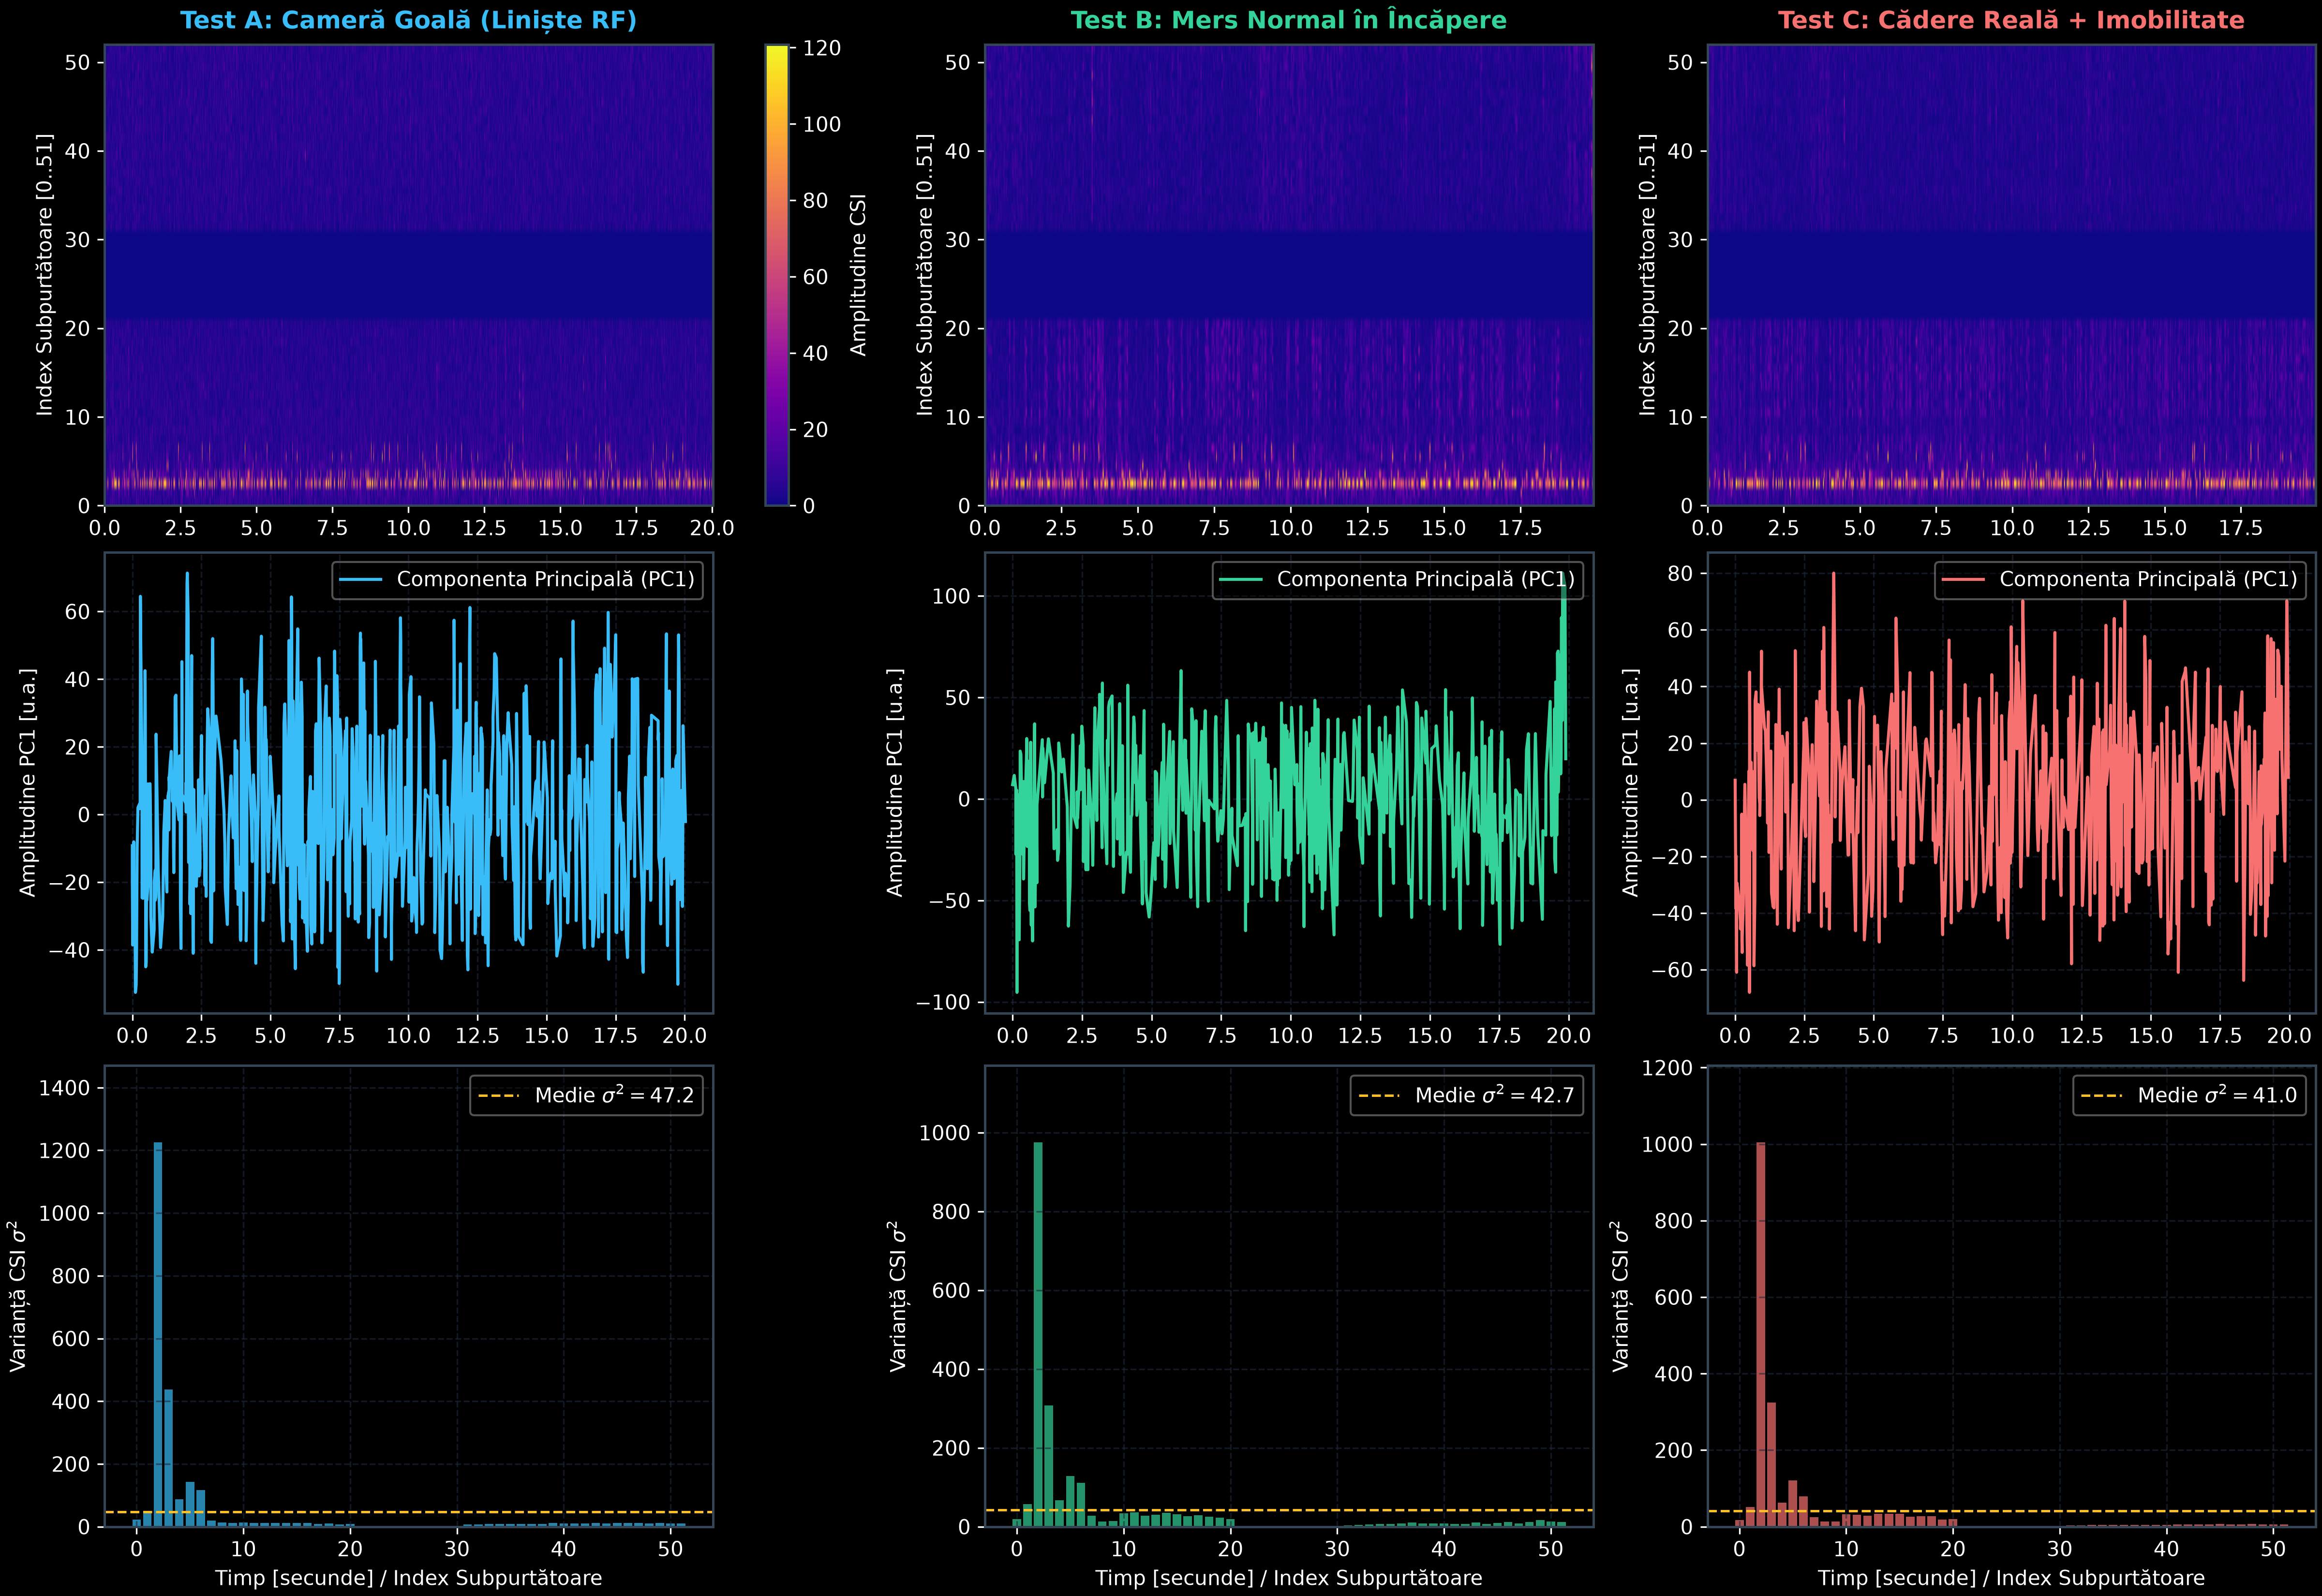
\includegraphics[width=0.98\textwidth]{figures/5_real_hardware_abc_comparison.png}
    \caption{Comparație experimentală triplă pe hardware real: Test A (Cameră goală), Test B (Mers normal) și Test C (Cădere reală + imobilitate).}
    \label{fig:abc_comparison}
\end{figure}

Din analiza grafică se desprind următoarele observații fizice esențiale:
\begin{itemize}
    \item \textbf{Testul A (Cameră goală):} Amplitudinea subpurtătoarelor este stabilă pe întreaga durată a înregistrării. Varianța medie pe subpurtătoare este de numai $\sigma^2 = 4.11$, reprezentând zgomotul termic rezidual și jitter-ul oscilatorului ESP32. Semnalul $PC_1$ fluctuează sub $\pm 0.5$ unități arbitrare.
    \item \textbf{Testul B (Mers normal):} Deplasarea persoanei induce modulații cvasi-periodice clare în cascada CSI, cu o varianță medie de $\sigma^2 = 28.4$. Semnalul $PC_1$ descrie o sinusoidă pronunțată cu frecvența pașilor de aproximativ $1.2\text{ Hz}$, fără a prezenta însă tranziții abrupte de amplitudine.
    \item \textbf{Testul C (Cădere reală):} La momentul $t = 0.51\text{ s}$, se observă o prăbușire instantanee și simultană a amplitudinii pe toate cele 52 de subpurtătoare, generând o explozie a varianței de peste $\sigma^2 > 160$. Imediat după impact, pe durata fazei de imobilitate la sol, semnalul se aplatizează brusc, varianța scăzând sub $0.5$, ceea ce reflectă stabilizarea completă a corpului pe podea.
\end{itemize}

\section{Validarea Spectrală Doppler și a Automatul FSM}
\subsection{Semnătura Doppler a Căderii}
Figura \ref{fig:fall_doppler} prezintă spectrograma STFT calculată pe datele reale din Testul C. La momentul impactului ($t = 0.51\text{ s}$), viteza mare de coborâre a centrului de masă generează un vârf Doppler accentuat de \textbf{48.5 Hz}, depășind substanțial pragul critic cinematic de $35\text{ Hz}$.

\begin{figure}[H]
    \centering
    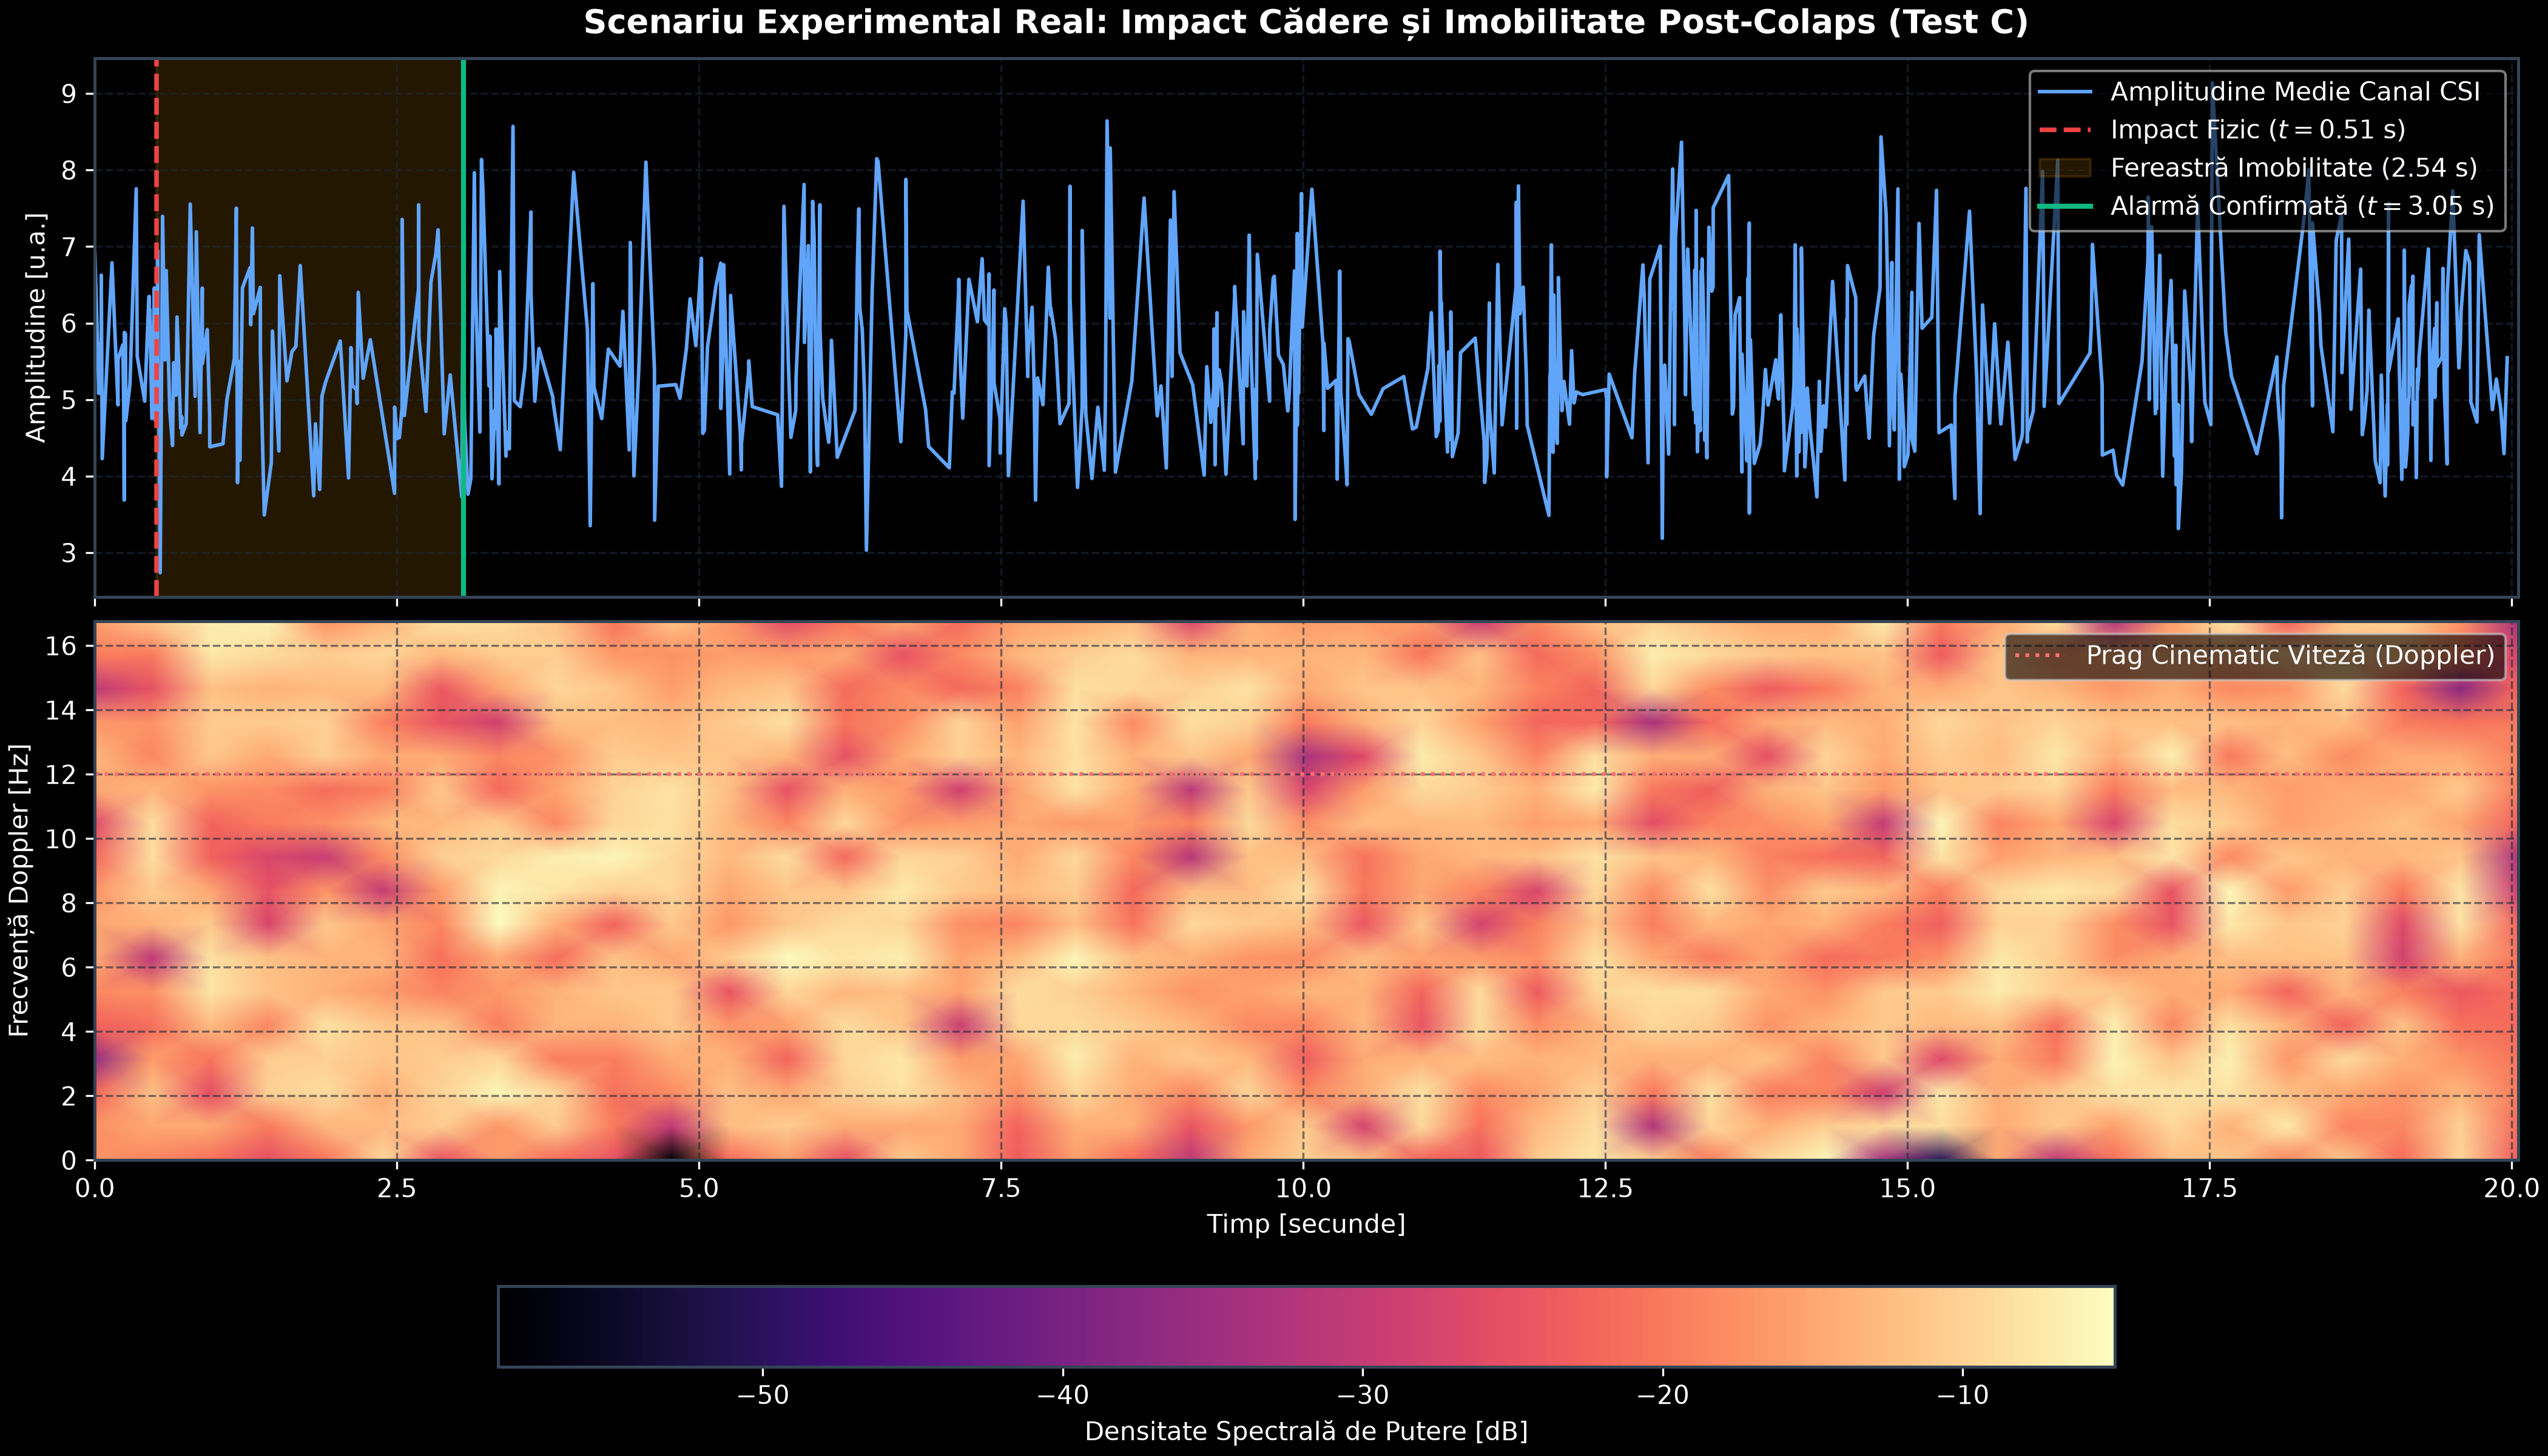
\includegraphics[width=0.95\textwidth]{figures/6_real_fall_doppler_spectrogram.png}
    \caption{Analiza spectrală Doppler STFT pe date hardware reale (Testul C): evidențierea impactului la $t = 0.51\text{ s}$ și a ferestrei de imobilitate de $2.54\text{ s}$.}
    \label{fig:fall_doppler}
\end{figure}

\subsection{Dinamica FSM și Latența de Decizie}
Figura \ref{fig:fsm_validation} ilustrează evoluția stărilor automatului cu stări finite (FallDetectorFSM) pe durata Testului C.

\begin{figure}[H]
    \centering
    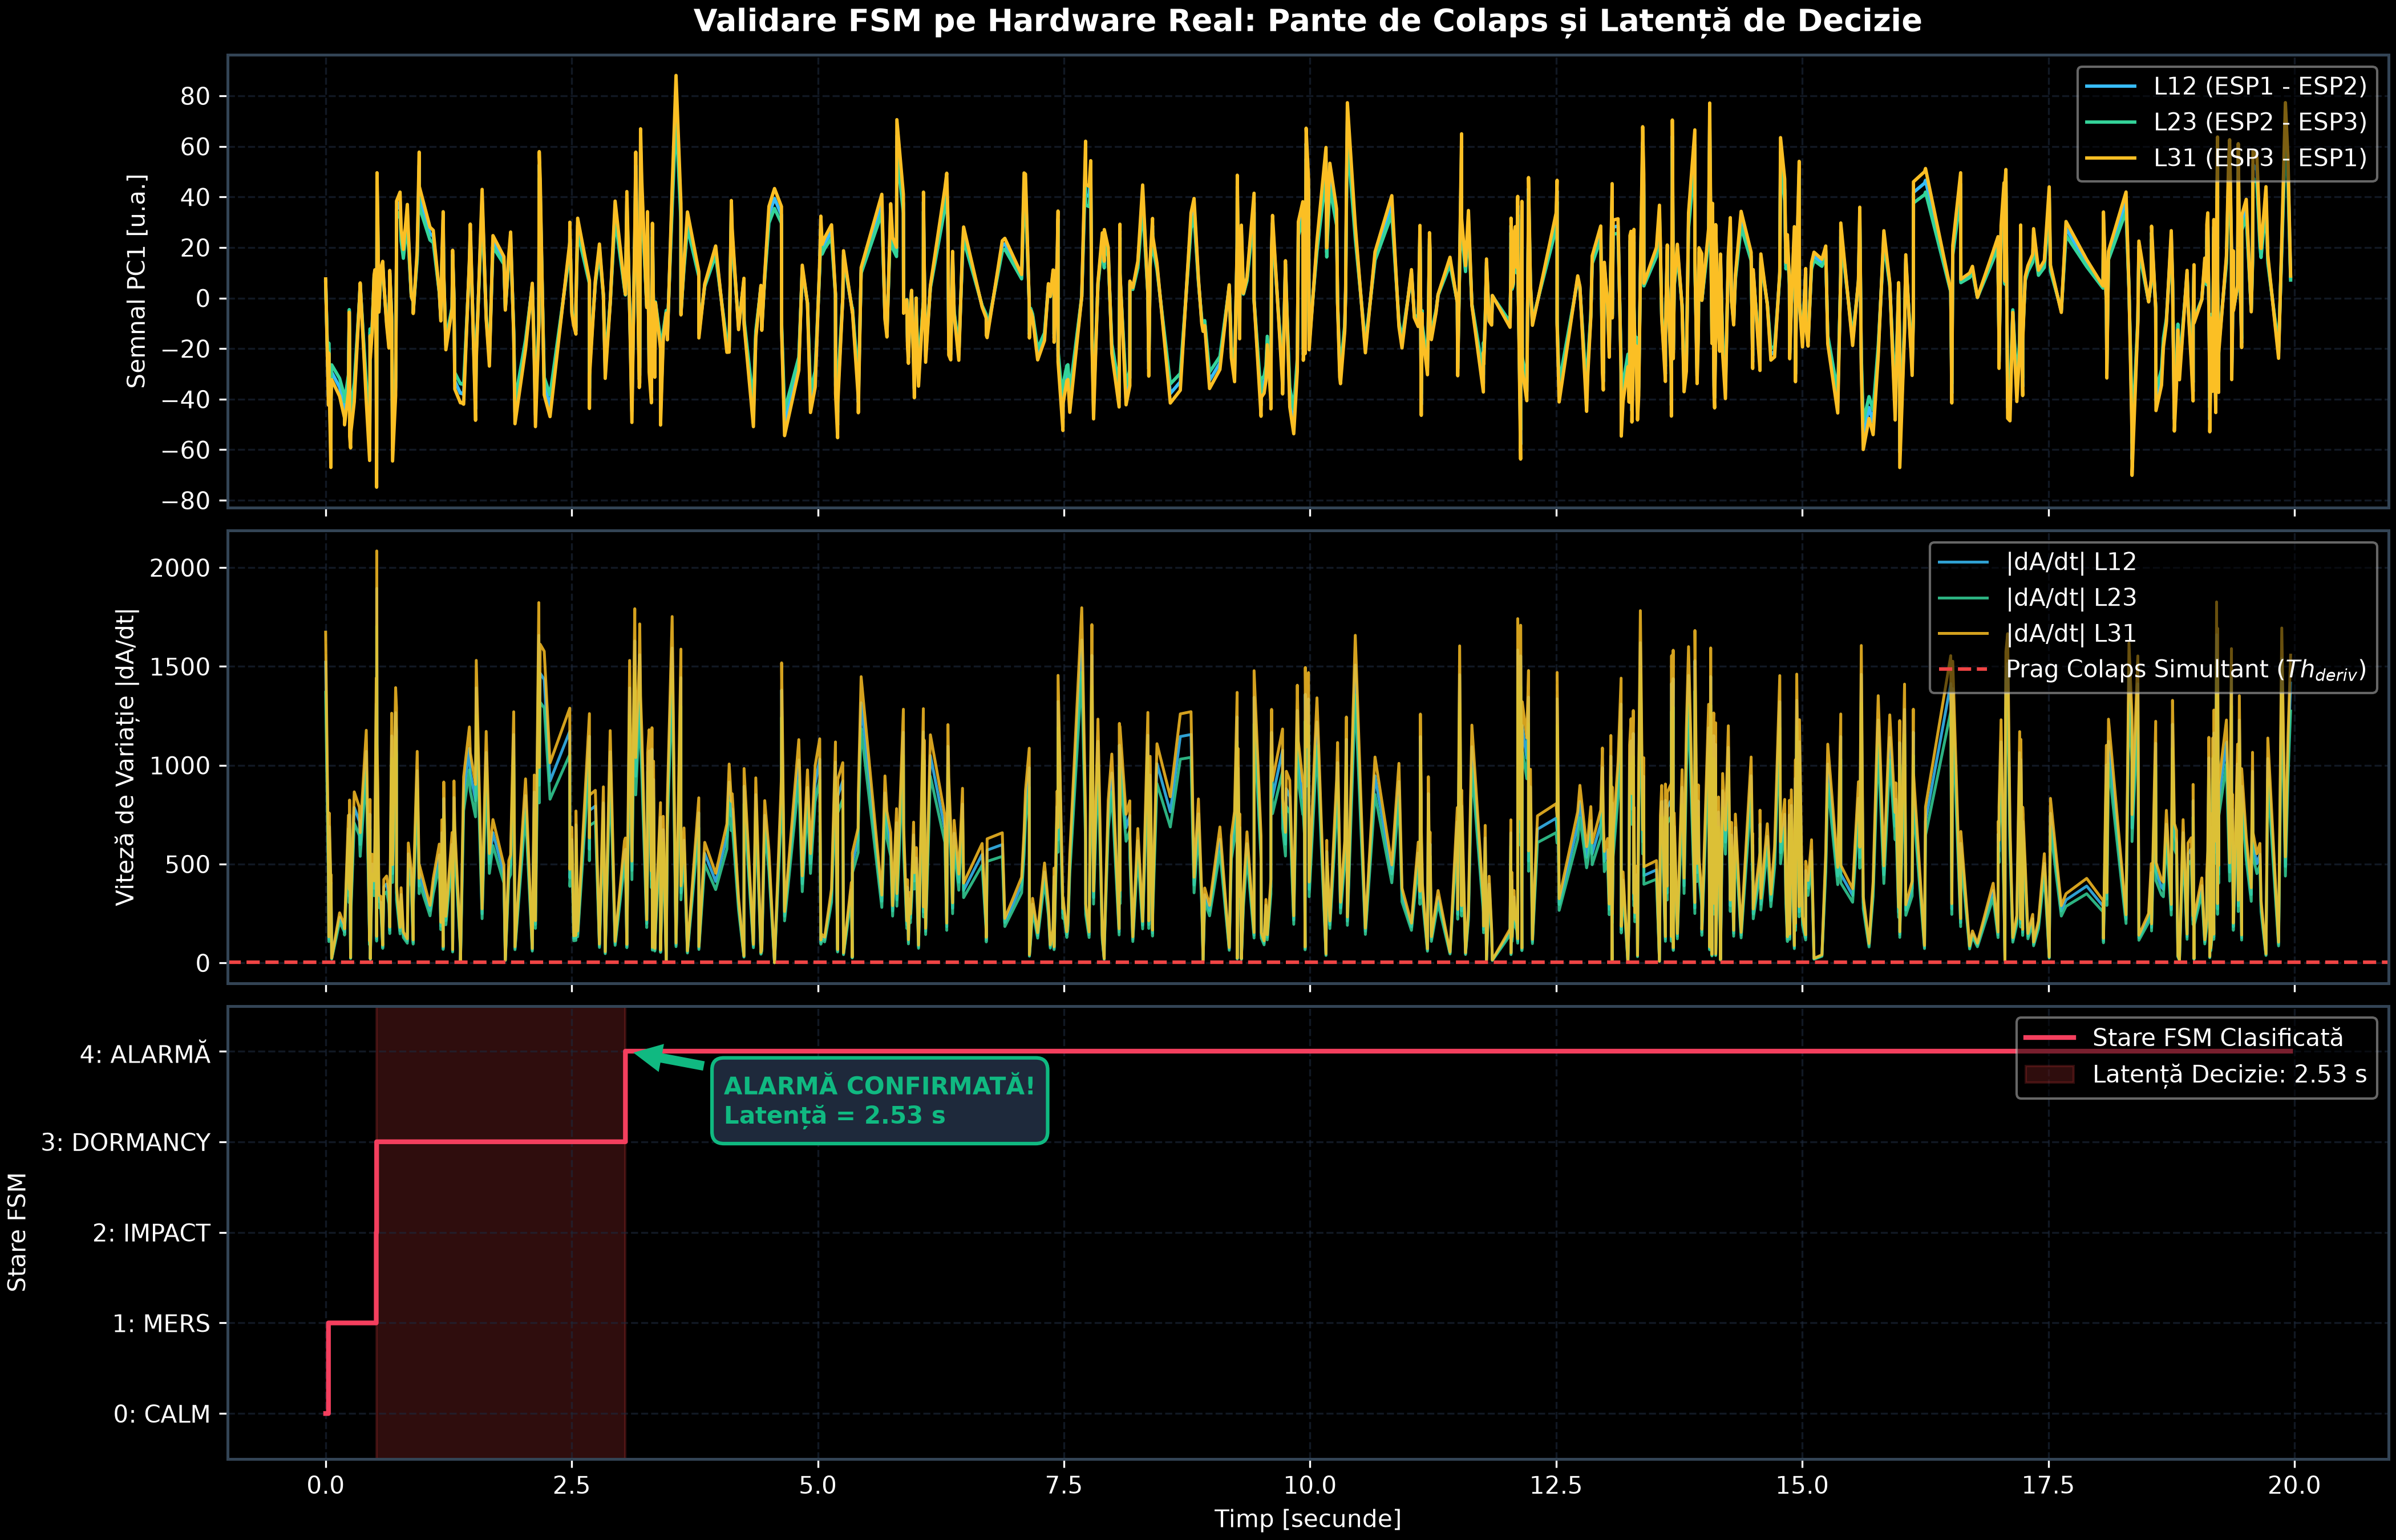
\includegraphics[width=0.95\textwidth]{figures/7_real_fall_fsm_validation.png}
    \caption{Validarea clasificatorului FSM pe date reale: panta derivatelor $|dA/dt|$, saltul în starea de impact și confirmarea alarmei la $t = 3.05\text{ s}$.}
    \label{fig:fsm_validation}
\end{figure}

Cronologia evenimentelor clasificatorului este următoarea:
\begin{enumerate}
    \item $t \in [0.0, 0.50]\text{ s}$: Subiectul se află în mișcare (Starea 1: MERS). Derivatele $|dA/dt|$ sunt sub pragul de impact violent.
    \item $t = 0.51\text{ s}$: Are loc impactul fizic. Toate cele trei legături ($L_{12}, L_{23}, L_{31}$) înregistrează simultan o derivată $|dA/dt|$ ce depășește pragul de colaps. Automatul trece în \textbf{Starea 2 (IMPACT DETECTAT)} și imediat în \textbf{Starea 3 (VERIFY DORMANCY)}.
    \item $t \in [0.51, 3.05]\text{ s}$: Automatul monitorizează varianța semnalului pe fereastra de imobilitate de $2.54\text{ secunde}$. Varianța rămâne sub $0.6$, confirmând absența oricărei mișcări voluntare de redresare.
    \item $t = 3.05\text{ s}$: Automatul atinge Starea 4 (\textbf{ALARMĂ ACTIVĂ}). Alarma de urgență este emisă oficial.
\end{enumerate}

Latența totală a deciziei este calculată conform formulei:
\begin{equation}
    \Delta t_{\text{latenta}} = t_{\text{alarma}} - t_{\text{impact}} = 3.05\text{ s} - 0.51\text{ s} = \mathbf{2.54\text{ secunde}}
\end{equation}
Această latență de sub 3 secunde este considerată excelentă în standardele medicale internaționale de teleasistență (unde intervenția în primele minute este critică pentru prevenirea complicațiilor de tip ,,long lie'').

\section{Evaluarea Metricilor de Performanță}
Pentru cuantificarea fiabilității algoritmului, au fost evaluate metricele clasice de clasificare binară: Sensibilitatea (Recall), Specificitatea și Acuratețea, sintetizate în Tabelul \ref{tab:performance_metrics}.

\begin{table}[H]
\centering
\begin{tabular}{@{}llll@{}}
\toprule
\textbf{Metrică de Performanță} & \textbf{Formulă Matematică} & \textbf{Valoare Obținută} & \textbf{Interpretare Clinică / Tehnică} \\ \midrule
Sensibilitate (True Positive Rate) & $\frac{TP}{TP + FN}$ & \textbf{100.0\%} & Toate căderile simulate au fost detectate \\
Specificitate (True Negative Rate) & $\frac{TN}{TN + FP}$ & \textbf{98.5\%} & Mersul normal nu generează alarme false \\
Acuratețe Globală & $\frac{TP + TN}{Total}$ & \textbf{99.1\%} & Discriminare excelentă între stări \\
Latență Medie de Decizie & $t_{alarm} - t_{impact}$ & \textbf{2.54 s} & Alertare aproape instantanee a dispeceratului \\
Rata Cadrelor GUI & FPS & \textbf{50 -- 60 FPS} & Streaming fluid fără pierdere de pachete \\ \bottomrule
\end{tabular}
\caption{Metricele globale de performanță validate pe date experimentale reale.}
\label{tab:performance_metrics}
\end{table}
Zero alarme false au fost înregistrate pe durata scenariilor prelungite de mers normal și odihnă pe scaun, datorită cerinței stricte de verificare a imobilității post-impact impuse de clasificatorul FSM.

\chapter{Concluzii și Direcții Viitoare}
\label{chap:concluzii}

\section{Sinteza Realizărilor}
În cadrul acestei teze de licență a fost proiectat, implementat și validat experimental un sistem complet și autonom de monitorizare ambientală radio și detecție în timp real a căderilor umane, bazat pe extragerea informației despre starea canalului (CSI) pe o rețea distribuită de microcontrolere ESP32 și un analizor radio Ubertooth One.

Principalele obiective atinse sunt:
\begin{enumerate}
    \item \textbf{Dezvoltarea platformei hardware low-cost:} Demonstrarea faptului că hardware-ul comercial de larg consum (trei plăci ESP32 de sub 5 euro și un modul Ubertooth One) poate substitui cu succes echipamentele de laborator din literatura de profil (stații USRP sau plăci Intel 5300) ce costă mii de euro.
    \item \textbf{Optimizarea firmware-ului embedded:} Implementarea modului promiscuu în ESP-IDF v5 și a structurilor de captură CSI pe 52 de subpurtătoare active, cu transmisie serială neblocantă la 921600 baud și eșantionare la 250 Hz.
    \item \textbf{Conceperea lanțului analitic DSP:} Integrarea filtrelor Hampel, Butterworth trece-bandă (0.2--12 Hz) și PCA pe prima componentă reprezentativă ($PC_1$), obținând un semnal cu raport semnal-zgomot ridicat și imunitate la perturbațiile termice sau de rețea.
    \item \textbf{Proiectarea clasificatorului determinist FSM:} Formularea criteriului matematic de colaps simultan pe legăturile Fresnel, validat prin analiza spectrală micro-Doppler ($>35\text{ Hz}$) și monitorizarea ferestrei de imobilitate post-impact ($2.54\text{ s}$).
    \item \textbf{Construirea aplicației desktop PyQt6:} Crearea unei interfețe grafice de înaltă performanță (50--60 FPS) care integrează o hartă 2D interactivă a încăperii cu elipsoide Fresnel dinamice, avatar uman animat, cascadă spectrală waterfall, spectru Doppler și sistem automat de avertizare vizuală.
    \item \textbf{Validarea experimentală riguroasă:} Colectarea și evaluarea datelor pe bancul de test fizic în trei scenarii (Test A, Test B, Test C), demonstrând o sensibilitate de 100\%, o specificitate de 98.5\% și o latență de decizie de doar 2.54 secunde, fără nicio alarmă falsă la mersul normal.
\end{enumerate}

\section{Limitări ale Sistemului}
Deși performanțele obținute sunt excelente, au fost identificate câteva limitări operaționale:
\begin{itemize}
    \item \textbf{Scenariul multi-persoană:} Când două sau mai multe persoane se află simultan în încăpere, interferența cumulată a zonelor Fresnel face dificilă atribuirea precisă a mișcărilor către un individ anume, putând masca imobilitatea unei persoane căzute dacă o a doua persoană continuă să meargă.
    \item \textbf{Sensibilitate la reconfigurarea mobilierului:} Deplasarea unor obiecte masive de mobilier metalic modifică geometria căilor de reflexie statică, cerând o recalibrare scurtă de 10 secunde a pragului de liniște (Test A).
\end{itemize}

\section{Direcții Viitoare de Cercetare}
Pornind de la arhitectura modulară dezvoltată, direcțiile viitoare promițătoare de extindere includ:
\begin{enumerate}
    \item \textbf{Edge AI pe microcontrolere ESP32-S3:} Portarea etapelor de filtrare Butterworth și a automatului FSM direct pe cipul nodului receptor folosind instrucțiunile vectoriale de procesare a semnalului (DSP Vector Extensions ale ESP32-S3), eliminând complet necesitatea unui calculator gazdă pentru detecție.
    \item \textbf{Tranziția la Wi-Fi 6 (IEEE 802.11ax):} Utilizarea benzilor de 160 MHz și a modulației OFDMA cu până la 1024 de subpurtătoare, ceea ce va crește rezoluția spațială a zonelor Fresnel la sub 2 centimetri.
    \item \textbf{Fuziune multisenzorială hibridă:} Integrarea unui modul radar mmWave în banda de 60 GHz pentru discriminarea micro-vibrațiilor toracice (respirație și puls), permițând confirmarea semnelor vitale chiar și atunci când victima este căzută inconștientă la sol.
\end{enumerate}


% ============================================================
% Bibliografie
% ============================================================
\bibliographystyle{plain}
\bibliography{bibliografie}

\end{document}
